% TouchSynth design report
% build: latexmk -pdf touchsynth_report.tex   (run python gen_tables.py first)
\documentclass[11pt,a4paper]{article}
\usepackage[T1]{fontenc}
\usepackage[utf8]{inputenc}
\usepackage{lmodern}
\usepackage{microtype}
\usepackage[a4paper,textwidth=16cm,top=2.5cm,bottom=2.7cm]{geometry}
\usepackage{graphicx}
\usepackage{booktabs,longtable,tabularx,array,multirow}
\usepackage{siunitx}
\usepackage{xcolor}
\usepackage{tikz}
\usetikzlibrary{positioning,arrows.meta,fit,calc,shapes.geometric}
\usepackage[siunitx,american]{circuitikz}
\usepackage{caption,subcaption}
\usepackage{enumitem}
\usepackage{pdfpages}
\usepackage{fancyhdr}
\usepackage[hidelinks]{hyperref}

\graphicspath{{../figures/}}
\captionsetup{font=small,labelfont=bf}
\setlist{nosep,leftmargin=1.4em}
\sisetup{range-phrase=\,\ldots\,,range-units=single}
\newcommand{\file}[1]{\texttt{#1}}
\newcommand{\sub}[1]{\textsubscript{#1}}
\newcommand{\statBomlines}{40}
\newcommand{\statPlaced}{196}
\newcommand{\statPartscost}{3.65}
\newcommand{\statBasiclines}{38}
\newcommand{\statPromolines}{2}
\newcommand{\statParts}{242}
\newcommand{\statNets}{166}
\newcommand{\statSheets}{7}
\newcommand{\statDnp}{5}


\pagestyle{fancy}
\fancyhf{}
\lhead{\small TouchSynth -- design report}
\rhead{\small rev 0.1}
\cfoot{\small\thepage}

\title{\textbf{TouchSynth}\\[4pt]\large An MCU-controlled analog monophonic synthesizer\\ on a single 4-layer board\\[10pt]
\normalsize Design report, revision 0.1}
\author{cpldcpu \and Claude Opus 5.5}
\date{27 September 2026}

\begin{document}
\maketitle
\thispagestyle{empty}

\begin{abstract}
\noindent TouchSynth is a small monophonic analog synthesizer that is played on a capacitive touch keyboard
and controlled entirely by a CH32V003/CH32V002 microcontroller. It has no potentiometers or mechanical
switches. The sound path is fully analog:
\begin{itemize}
  \item a timer-reset integrator oscillator (DCO),
  \item a four-pole transistor ladder filter with voltage-controlled resonance,
  \item a BJT differential-pair VCA with a firmware-calibrated offset trim.
\end{itemize}
All control voltages are generated by PWM and passive filters. The board uses only JLCPCB \emph{Basic} and
\emph{Promotional Extended} parts; the MCU is hand-soldered from own stock.

This report documents the requirements, the circuit design and its justification by ngspice simulation
(seven blocks plus the complete voice), a behavioural audio model, the 4-layer PCB, the bill of materials
and the verification and validation plan, with the bring-up and functional test results of the first assembled
board.
\end{abstract}

\vspace{1em}
\begin{figure}[h]
  \centering
  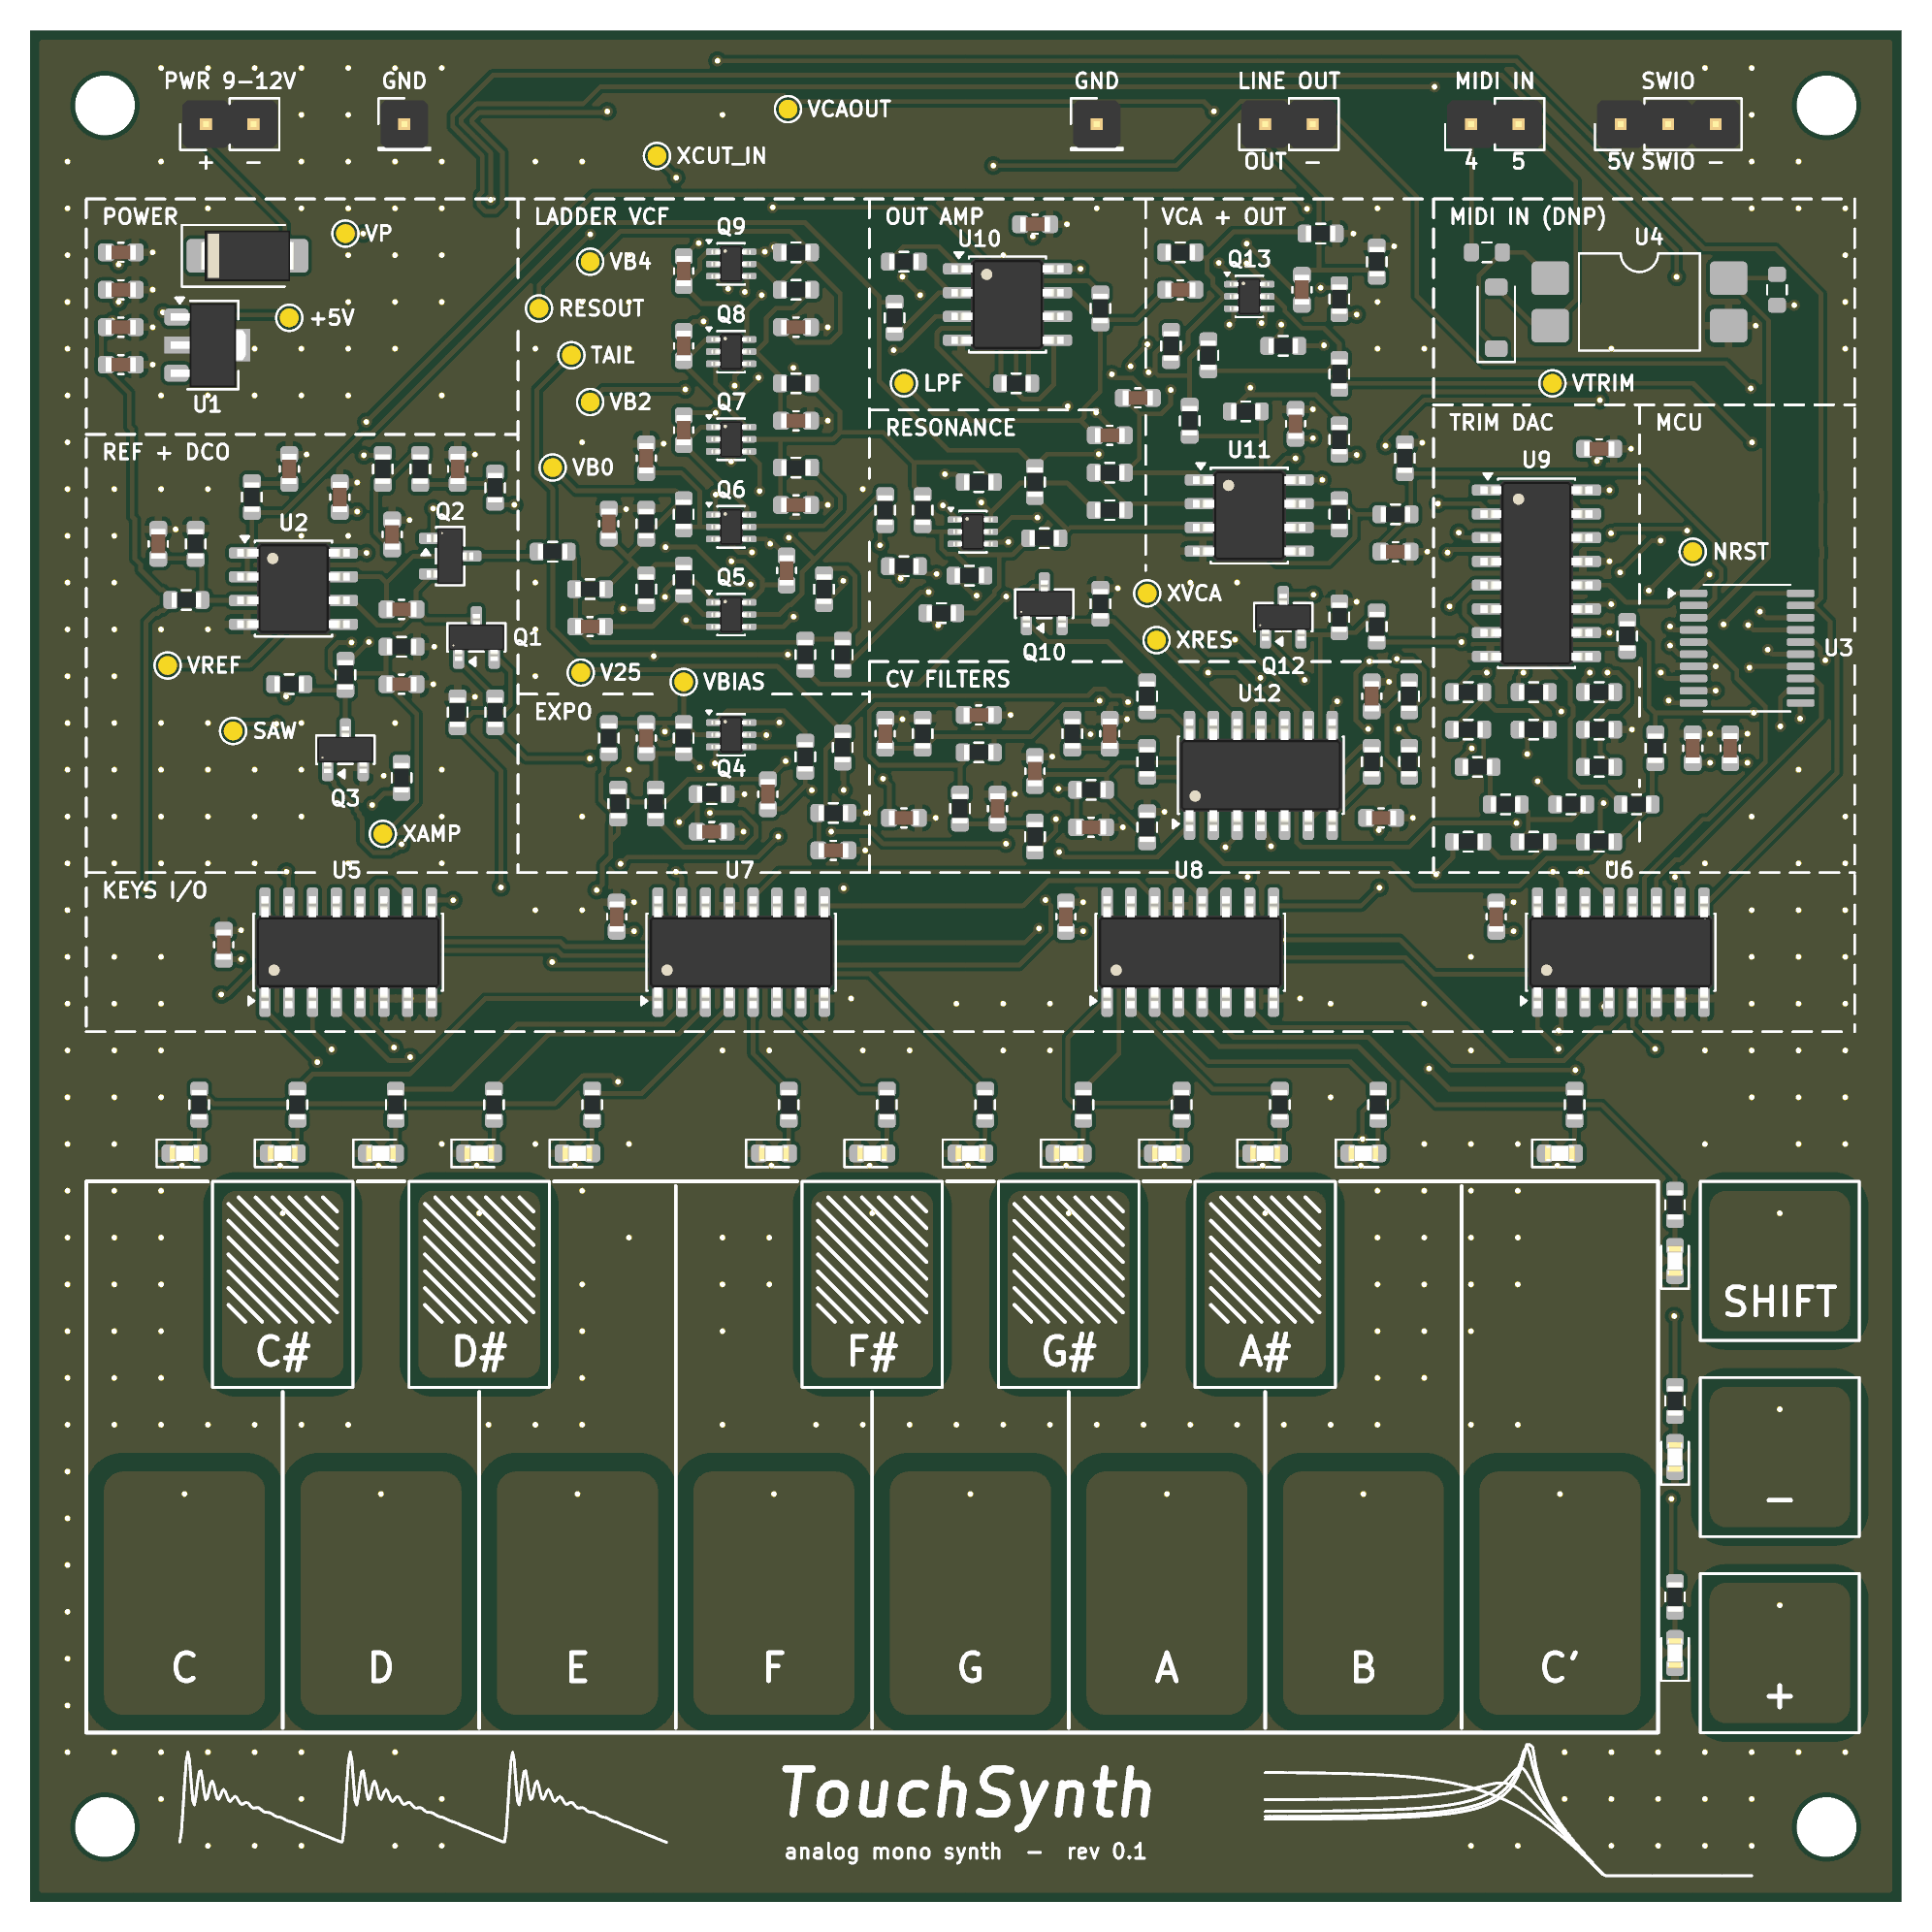
\includegraphics[width=0.62\textwidth]{pcb/render_top.png}
  \caption{The board as ordered (rendered in KiCad 10), 100 $\times$ 100\,mm, 4 layers.}
  \label{fig:hero}
\end{figure}

\clearpage
\tableofcontents
\clearpage

% =====================================================================================================
\section{Introduction}

\subsection{Goal and constraints}
The project had three aims:
\begin{enumerate}
  \item Design a complete, self-contained electronic instrument end to end: requirements, circuit design,
    simulation, PCB layout and fabrication.
  \item Keep the part count and the cost of assembly low.
  \item Build in enough observability that the board can be verified automatically once it is back from
    the factory.
\end{enumerate}
The following constraints shaped the design:
\begin{itemize}
  \item \textbf{Parts}: only JLCPCB \emph{Basic} and \emph{Promotional Extended} parts, so there are no
    feeder loading fees and the board can be assembled in JLCPCB's economic PCBA service. The part lists
    were downloaded from the JLCPCB parts API (351 Basic and 1235 Promotional parts) and every BOM line was
    chosen from them.
  \item \textbf{MCU}: a CH32V003F4P6 or CH32V002F4P6 in TSSOP-20 from own stock, hand-soldered
    (do-not-populate in the assembly BOM). Both variants are pin compatible; one firmware supports both.
  \item \textbf{User interface}: no potentiometers and no mechanical switches. Thirteen capacitive keys
    (one octave C--C) plus three function pads (SHIFT, $-$, $+$), and 16 LEDs.
  \item \textbf{Power}: \SIrange{9}{12}{V} DC on a 2-pin header, reverse-polarity protected.
  \item \textbf{Scope}: a demonstrator. Some imperfections (power-on pop, filter temperature drift) are
    accepted explicitly rather than solved with additional parts. MIDI input is laid out but not populated.
\end{itemize}

\subsection{Tool flow}
The design was carried out with open tools and scripts, so every artefact can be regenerated
(Table~\ref{tab:tools}). A single Python description of the circuit (\file{hw/design.py}) is the source of
truth: the schematic, the PCB netlist and the simulation cross-check are all derived from it.

\begin{table}[h]
\centering\small
\caption{Tool flow and where each step lives in the repository.}\label{tab:tools}
\begin{tabularx}{\textwidth}{@{}>{\raggedright}p{2.7cm} >{\raggedright}p{4.4cm} >{\raggedright\arraybackslash}X@{}}
\toprule
Step & Tool & Files \\
\midrule
Part selection & JLCPCB parts API & \file{parts/*.csv} \\
Circuit simulation & ngspice-42 (WSL), Python & \file{sim/s1\_dco} \ldots\ \file{sim/s7\_power}, \file{sim/lib/voice.py} \\
Behavioural audio model & Python + numba & \file{sim/behav/} \\
Circuit description & Python & \file{hw/design.py} (\statParts\ parts, \statNets\ nets) \\
Schematic & generated KiCad 10 schematic & \file{gen\_sch2.py}, \file{layouts.py}, \file{draw.py} (in \file{hw/}) \\
Checks & kicad-cli ERC, netlist and simulation cross-check & \file{check\_netlist.py}, \file{check\_sim.py} (in \file{hw/}) \\
PCB & KiCad 10 Python API, Freerouting 1.9, own maze router & \file{hw/gen\_pcb.py}, \file{hw/pcb\_*.py} \\
Fabrication data & kicad-cli & \file{hw/fab.py} \\
Firmware & ch32fun (git submodule), riscv64-unknown-elf-gcc & \file{firmware/} \\
\bottomrule
\end{tabularx}
\end{table}

% =====================================================================================================
\section{Requirements}

Table~\ref{tab:req} summarises the functional requirements (full text in \file{docs/spec.md}). Each
requirement is traced to a simulation and to a hardware test in Section~\ref{sec:vv}.

\begin{table}[h]
\centering\small
\caption{Functional requirements.}\label{tab:req}
\begin{tabularx}{\textwidth}{@{}l X@{}}
\toprule
Block & Requirement \\
\midrule
DCO & Pitch from an MCU timer, range $\geq$ C1 (\SI{32.7}{Hz}) \ldots\ C7 (\SI{2093}{Hz}); saw amplitude
constant within $\pm$\SI{5}{\percent} over the range \\
Waveforms & saw, pulse with variable width, sub-oscillator ($-1$ octave square), noise; each switchable \\
VCF & 24\,dB/oct transistor ladder; cutoff \SIrange{30}{15000}{Hz} via a hardware exponential converter;
resonance from zero to self-oscillation \\
VCA & $\geq$ \SI{70}{dB} attenuation when closed; envelope from firmware; CV feed-through nulled by a
calibrated trim \\
Output & line level $\approx$ \SI{1}{V_{pp}} into $\geq$ \SI{10}{k\ohm}, AC coupled \\
Control voltages & 4 PWM channels, 12-bit effective resolution; ripple $<$ \SI{-70}{dB} of full scale;
settling $<$ \SI{2}{ms} \\
Touch & 16 pads; full scan $\geq$ \SI{200}{Hz}; touch signal $\geq 5\times$ noise \\
Power & \SIrange{9}{12}{V}, reverse protected, $\leq$ \SI{60}{mA} \\
Test & audio loopback to the MCU ADC; test points; programming/debug over SWIO \\
\bottomrule
\end{tabularx}
\end{table}

% =====================================================================================================
\section{System architecture}

Figure~\ref{fig:block} shows the architecture:
\begin{itemize}
  \item \textbf{Audio path} (top row): analog from the oscillator to the line output.
  \item \textbf{MCU}: generates the oscillator timing and the waveform bits directly. The four continuous
    parameters (oscillator amplitude, cutoff, resonance, VCA level) are PWM outputs of TIM1, smoothed by
    passive three-pole filters and converted to currents.
  \item \textbf{Touch pads}: read through two CD4051 multiplexers with the ADC charge-slope method.
  \item \textbf{Shift-register chain}: three 74HC595 drive the 16 LEDs and an 8-bit R-2R DAC that trims
    the VCA offset.
  \item \textbf{Loopback}: a divided copy of the output returns to an ADC pin. It is used for
    self-test and calibration.
\end{itemize}

\begin{figure}[ht]
\centering
\resizebox{\textwidth}{!}{%
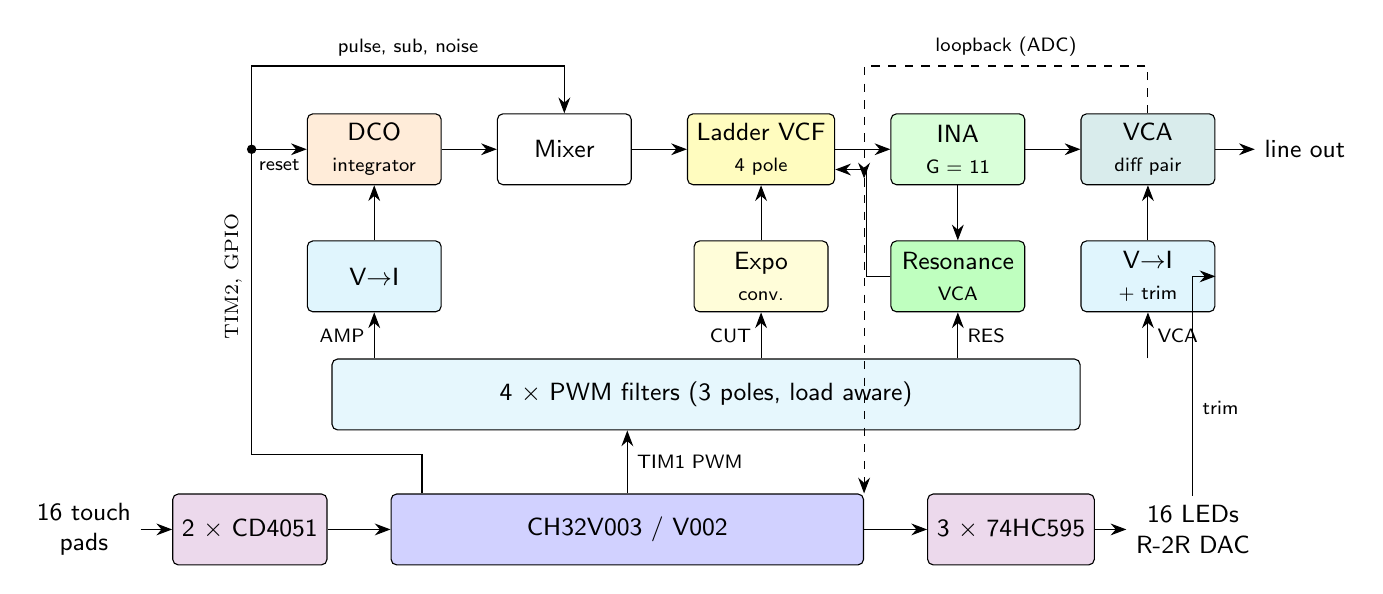
\begin{tikzpicture}[font=\small\sffamily, node distance=6mm and 7mm,
  blk/.style={draw, rounded corners=2pt, fill=#1, minimum height=9mm, minimum width=17mm, align=center},
  blk/.default=white, >={Stealth[length=2mm]}]
  \node[blk=orange!15] (dco) {DCO\\\scriptsize integrator};
  \node[blk=white, right=of dco] (mix) {Mixer};
  \node[blk=yellow!25, right=of mix] (vcf) {Ladder VCF\\\scriptsize 4 pole};
  \node[blk=green!15, right=of vcf] (ina) {INA\\\scriptsize G = 11};
  \node[blk=teal!15, right=of ina] (vca) {VCA\\\scriptsize diff pair};
  \node[right=5mm of vca] (out) {line out};
  \node[blk=green!25, below=7mm of ina] (res) {Resonance\\\scriptsize VCA};
  \node[blk=yellow!15, below=7mm of vcf] (expo) {Expo\\\scriptsize conv.};
  \node[blk=cyan!12, below=7mm of dco] (vi1) {V$\to$I};
  \node[blk=cyan!12, below=7mm of vca] (vi3) {V$\to$I\\\scriptsize + trim};
  \node[blk=cyan!10, below=22mm of mix, minimum width=95mm, xshift=18mm] (cvf) {4 $\times$ PWM filters (3 poles, load aware)};
  \node[blk=blue!18, below=8mm of cvf, minimum width=60mm, xshift=-10mm] (mcu) {CH32V003 / V002};
  \node[blk=violet!15, left=8mm of mcu] (mux) {2 $\times$ CD4051};
  \node[left=4mm of mux, align=center] (pads) {16 touch\\pads};
  \node[blk=violet!15, right=8mm of mcu] (sr) {3 $\times$ 74HC595};
  \node[right=4mm of sr, align=center] (leds) {16 LEDs\\R-2R DAC};
  \draw[->] (dco) -- (mix); \draw[->] (mix) -- (vcf); \draw[->] (vcf) -- (ina); \draw[->] (ina) -- (vca);
  \draw[->] (vca) -- (out);
  \draw[->] (ina.south) -- (res.north); \draw[->] (res.west) -- ++(-3mm,0) |- ($(vcf.south east)+(0,2mm)$);
  \draw[->] (expo) -- (vcf);
  \draw[->] (vi1) -- (dco);
  \draw[->] (vi3) -- (vca);
  \draw[->] (cvf.north -| vi1) -- (vi1) node[pos=0.5,left] {\scriptsize AMP};
  \draw[->] (cvf.north -| expo) -- (expo) node[pos=0.5,left] {\scriptsize CUT};
  \draw[->] (cvf.north -| res.south) -- (res.south) node[pos=0.5,right] {\scriptsize RES};
  \draw[->] (cvf.north -| vi3) -- (vi3) node[pos=0.5,right] {\scriptsize VCA};
  \draw[->] (mcu.north) -- (mcu.north |- cvf.south) node[pos=0.5,right] {\scriptsize TIM1 PWM};
  \draw[->] (pads) -- (mux); \draw[->] (mux) -- (mcu); \draw[->] (mcu) -- (sr); \draw[->] (sr) -- (leds);
  % timing / waveform lines: up a lane left of the analog blocks; reset to the DCO, pulse/sub/noise to the mixer
  \coordinate (lane) at ($(dco.west)+(-7mm,0)$);
  \draw[->] ($(mcu.north west)+(4mm,0)$) -- ++(0,5mm) -| (lane) -- (dco.west) node[pos=0.5,below] {\scriptsize reset};
  \draw[->] (lane) |- ($(mix.north)+(0,6mm)$) node[pos=0.75,above] {\scriptsize pulse, sub, noise} -- (mix.north);
  \fill (lane) circle (0.6mm);
  \node[font=\scriptsize, rotate=90, anchor=south] at ($(lane |- vi1)+(0,0)$) {TIM2, GPIO};
  \draw[->,dashed] (vca.north) -- ++(0,6mm) -| ($(mcu.north east)+(0,40mm)$) node[pos=0.25,above] {\scriptsize loopback (ADC)};
  \draw[->,dashed] ($(mcu.north east)+(0,40mm)$) -- ($(mcu.north east)+(0,0)$);
  \draw[->] (leds.north) |- (vi3.east) node[pos=0.2,right] {\scriptsize trim};
\end{tikzpicture}}
\caption{System architecture. The audio path is analog; the MCU sets all parameters through PWM control voltages
and timing, and observes the output through the loopback.}
\label{fig:block}
\end{figure}

\subsection{Control concept}
\begin{itemize}
  \item \textbf{Oscillator timing}: TIM2 CH1 produces one short reset pulse per period, so the pitch is as
    exact as the \SI{48}{MHz} timer. The saw amplitude is kept constant by making the integrator charging
    current proportional to the frequency (CV\sub{AMP}).
  \item \textbf{Waveform bits}: the pulse wave comes from TIM2 CH2. The sub-oscillator is a GPIO toggled in
    the TIM2 update interrupt, and noise is a GPIO driven by a firmware LFSR.
  \item \textbf{Control voltages}: TIM1 CH1--CH4 run at 10 bit and \SI{46.9}{kHz}. The compare registers
    are updated by DMA bursts with 2-bit sigma-delta dithering, which gives 12-bit effective resolution at
    a high carrier frequency.
  \item \textbf{Firmware control loop}: envelopes, LFO, glide and the arpeggiator run in firmware at a
    \SI{1}{kHz} control rate.
\end{itemize}

\subsection{MCU pin assignment}
Table~\ref{tab:pins} lists the pin map. The LED/DAC shift registers share the DATA and CLOCK lines with the
multiplexer select lines S0 and S1, so no third multiplexer is needed.

\begin{table}[h]
\centering\small
\caption{MCU pin map (TSSOP-20, identical for CH32V003 and CH32V002).}\label{tab:pins}
\begin{tabular}{@{}r l l @{\hspace{2em}} r l l@{}}
\toprule
Pin & Port & Function & Pin & Port & Function \\
\midrule
1 & PD4 & 74HC595 LATCH & 11 & PC1 & SUB oscillator (GPIO) \\
2 & PD5 & ADC A5 $\leftarrow$ audio loopback & 12 & PC2 & TIM2 CH2 $\to$ PULSE \\
3 & PD6 & USART RX $\leftarrow$ MIDI & 13 & PC3 & mux S0 / 595 DATA \\
4 & PD7 & NRST & 14 & PC4 & mux S1 / 595 CLK \\
5 & PA1 & touch mux B $\to$ ADC A1 & 15 & PC5 & TIM2 CH1 $\to$ DCO reset \\
6 & PA2 & touch mux A $\to$ ADC A0 & 16 & PC6 & TIM1 CH1 $\to$ CV\sub{AMP} \\
7 & VSS & GND & 17 & PC7 & TIM1 CH2 $\to$ CV\sub{CUT} \\
8 & PD0 & NOISE (GPIO) & 18 & PD1 & SWIO \\
9 & VDD & +5\,V & 19 & PD2 & mux S2 \\
10 & PC0 & TIM1 CH3 $\to$ CV\sub{RES} & 20 & PD3 & TIM1 CH4 $\to$ CV\sub{VCA} \\
\bottomrule
\end{tabular}
\end{table}

% =====================================================================================================
\section{Circuit design}\label{sec:circuit}

The complete schematic (7 hierarchical sheets) is reproduced in Appendix~\ref{app:sch}. This section explains
each block and its key values. Unless noted, all resistors are \SI{1}{\percent} thick film 0603, and all
capacitors are X7R/X5R 0603.

\subsection{Power and references}
\begin{itemize}
  \item \textbf{Input}: an SS14 Schottky diode protects against reverse polarity. The protected rail V+
    (\SIrange{8.6}{11.6}{V}) supplies the analog circuitry.
  \item \textbf{+5\,V}: a 78L05 supplies the MCU, the multiplexers, the shift registers and the LEDs.
  \item \textbf{Audio reference}: VREF = \SI{4.5}{V} is derived from +5\,V (\SI{1}{k\ohm}/\SI{9.1}{k\ohm}
    divider, \SI{10}{\micro F}) and buffered by a TL072 follower. The follower has a
    \SI{10}{\ohm}\,+\,\SI{1}{\micro F} output snubber instead of a bare capacitor. The simulation showed
    that the snubber is required for stability, see Section~\ref{sec:sim}.
  \item \textbf{Other references}: VBIAS = \SI{1.5}{V} and V25 = \SI{2.5}{V} are plain dividers from +5\,V.
    Referencing everything that sets pitch or cutoff to +5\,V, not to V+, makes the sound independent of
    the input voltage.
\end{itemize}

\subsection{Oscillator (DCO)}
The oscillator is a TL072 inverting integrator ($C_\mathrm{int}$ = \SI{10}{nF}) whose non-inverting input sits at
VREF (Figure~\ref{fig:dco}):
\begin{itemize}
  \item \textbf{Charging}: a V$\to$I converter (LM324 + MMBT3904, $R_E$ = \SI{33}{k\ohm}) draws the
    charging current from the summing node, so the saw ramps up from \SI{4.5}{V}.
  \item \textbf{Reset}: once per period a \SI{3}{\micro s} pulse from TIM2 CH1 goes through an MMBT3904
    level shifter to a 2N7002 across the capacitor. A \SI{2.2}{k\ohm} gate resistor softens the
    charge-injection spike.
  \item \textbf{Constant amplitude}: the firmware sets
    $I = A\,C_\mathrm{int}/(T - t_\mathrm{reset})$, so the saw amplitude $A$ does not depend on the
    period $T$.
\end{itemize}

\begin{figure}[ht]
\centering
\begin{circuitikz}[scale=0.85, transform shape, font=\small]
  \draw (0,0) node[op amp](OA){\scriptsize TL072};
  \draw (OA.-) -- ++(-1.2,0) coordinate(N);
  \draw (N) -- ++(0,1.6) coordinate(T) to[C, l=$C_\mathrm{int}$ 10\,nF] (T -| OA.out) -- (OA.out);
  \draw (T) -- ++(0,1.4) coordinate(T2) to[nos, l={2N7002 reset (TIM2 CH1 via level shifter)}] (T2 -| OA.out) -- ++(0,-1.4);
  \draw (N) to[american current source, l_={$I \propto f$ (CV\sub{AMP})}] ++(0,-2.6) node[ground]{};
  \draw (OA.+) -- ++(-0.5,0) -- ++(0,-1.1) node[right]{$V_\mathrm{REF}$ = 4.5\,V};
  \draw (OA.out) -- ++(1.2,0) node[right]{SAW \SIrange{4.5}{6.5}{V}};
  \node[align=right, font=\scriptsize, anchor=east] at ($(N)+(-0.5,-2.0)$) {V$\to$I: LM324 + MMBT3904,\\ $R_E$ = 33\,k$\Omega$};
\end{circuitikz}
\caption{DCO core (simplified): integrator with current-sink charging and a MOSFET reset switch.}
\label{fig:dco}
\end{figure}

\paragraph{Mixer.} The saw (\SI{150}{k\ohm}), pulse, sub and noise (\SI{470}{k\ohm} each) are summed into
\SI{10}{k\ohm} to the ladder input bias VB0 through \SI{1}{\micro F}.

\subsection{Control-voltage filters}
Each TIM1 PWM output is smoothed by three RC poles (Figure~\ref{fig:cvf}):
\begin{itemize}
  \item \textbf{LIN networks} (CV\sub{AMP}, CV\sub{RES}, CV\sub{VCA}): the last stage is a
    \SI{4.7}{k\ohm}/\SI{15}{k\ohm}\,$\|$\,\SI{22}{nF} divider into an LM324 V$\to$I converter.
    The DC ratio is 0.591.
  \item \textbf{EXP network} (CV\sub{CUT}): the last stage is a \SI{33}{k\ohm}/\SI{1.5}{k\ohm}\,$\|$\,\SI{100}{nF}
    divider to VBIAS. It drives the exponential converter base directly, with a ratio of 0.0373
    (10.4 octaves over the \SI{5}{V} PWM range).
\end{itemize}
Both ratios include the series resistance of the first two stages; Section~\ref{sec:lesson} describes the bug
that made this explicit.

\begin{figure}[ht]
\centering
\begin{circuitikz}[scale=0.85, transform shape, font=\small]
  \draw (0,0) node[left]{PWM (TIM1)} to[R, l=1\,k$\Omega$, o-*] (2.6,0)
        to[R, l=4.7\,k$\Omega$, -*] (5.2,0) to[R, l=4.7\,k$\Omega$, -*] (7.8,0) -- (9.2,0) node[circ]{}
        -- (10.2,0) node[right]{to LM324 V$\to$I};
  \draw (2.6,0) to[C, l_=100\,nF] (2.6,-2) node[ground]{};
  \draw (5.2,0) to[C, l_=33\,nF] (5.2,-2) node[ground]{};
  \draw (7.8,0) to[R, l_=15\,k$\Omega$] (7.8,-2) node[ground]{};
  \draw (9.2,0) to[C, l=22\,nF] (9.2,-2) node[ground]{};
\end{circuitikz}
\caption{LIN control-voltage network. The EXP variant (CV\sub{CUT}) replaces the last stage by
\SI{33}{k\ohm} / \SI{1.5}{k\ohm}\,$\|$\,\SI{100}{nF} to VBIAS.}
\label{fig:cvf}
\end{figure}

\subsection{Ladder filter, exponential converter and output amplifier}
\begin{itemize}
  \item \textbf{Ladder}: a Moog-type ladder made of five BC847BS dual NPN transistors (input pair, three
    rungs, load pair) and four \SI{33}{nF} capacitors.
  \item \textbf{Bias chain}: a divider from V+ (\SI{2.2}{k\ohm}, $4\times$\SI{1}{k\ohm}, \SI{2.4}{k\ohm},
    each tap decoupled with \SI{10}{\micro F}) sets the base voltages VB0 \ldots\ VB4.
  \item \textbf{Exponential converter}: the tail current comes from a BC847BS pair with an LM324. The
    reference current is \SI{8.3}{\micro A} through \SI{300}{k\ohm}, and the loop is compensated with
    \SI{1}{nF}.
  \item \textbf{Output amplifier}: the differential output across the top capacitor is read by a TL072
    two-op-amp instrumentation amplifier (gain 11, output referenced to VREF). Its JFET inputs do not load
    the ladder, whose source impedance reaches about \SI{50}{k\ohm} at low cutoff.
\end{itemize}

\subsection{Resonance}
The resonance loop is a voltage-controlled amplifier of its own:
\begin{itemize}
  \item \textbf{Input}: the filter output is attenuated 1:13 and AC coupled into a BC847BS differential
    pair.
  \item \textbf{Gain control}: the pair's tail current comes from CV\sub{RES} through an LM324 V$\to$I
    converter ($R_E$ = \SI{6.2}{k\ohm}).
  \item \textbf{Feedback}: the collectors feed a TL072 unity difference amplifier. Its output returns
    through \SI{4.7}{\micro F} and \SI{22}{k\ohm} into the second input of the ladder.
\end{itemize}
The difference amplifier removes the common-mode step of the collectors when the tail current changes. An
earlier single-ended version injected volt-level DC steps into the ladder.

\subsection{VCA, trim DAC and output}
\begin{itemize}
  \item \textbf{Core}: a BC847BS differential pair (bases biased from VREF, input attenuated 1:34) with
    \SI{4.7}{k\ohm} collector resistors. A TL072 difference amplifier (\SI{10}{k\ohm}/\SI{22}{k\ohm})
    follows, then \SI{10}{\micro F} to the line output.
  \item \textbf{Tail current}: an LM324 V$\to$I converter ($R_E$ = \SI{4.7}{k\ohm}) supplies it. A
    \SI{470}{k\ohm} resistor from +5\,V to the emitter makes the current truly zero at CV = 0 despite the
    op-amp offset voltage.
  \item \textbf{Offset trim}: the third 74HC595 in the LED chain drives an 8-bit R-2R DAC
    (\SI{100}{k\ohm}/\SI{200}{k\ohm}). The DAC injects a small offset current into one base
    (\SI{1}{M\ohm}, with \SI{2}{M\ohm} fixed on the other base). The firmware finds the DAC code that nulls
    the CV feed-through ("thump").
  \item \textbf{Loopback}: a \SI{10}{k\ohm}/\SI{15}{k\ohm} divider with \SI{1}{nF} feeds the output to PD5
    (ADC A5).
\end{itemize}

\subsection{Touch keyboard, LEDs and MIDI}
\begin{itemize}
  \item \textbf{Touch pads}: the 16 pads are copper under solder mask (white keys
    \SI{8.6}{mm}\,$\times$\,\SI{13}{mm}, black keys \SI{6.5}{mm}\,$\times$\,\SI{10}{mm}, function pads
    \SI{7.5}{mm} square). Each group of eight goes through a CD4051 to one ADC channel.
  \item \textbf{Measurement}: the ch32fun ADC slope method (\file{extralibs/ch32v00x\_touch.h}) measures
    each pad.
  \item \textbf{LEDs}: each of the 16 red 0603 LEDs has its own \SI{4.7}{k\ohm} series resistor (about
    \SI{0.6}{mA}).
  \item \textbf{MIDI}: an LTV-817 optocoupler feeds the USART RX pin. These parts are not populated; the
    footprints are kept.
\end{itemize}

% =====================================================================================================
\section{Simulation}\label{sec:sim}

\subsection{Method}
\begin{itemize}
  \item \textbf{Simulator}: every block was simulated in ngspice-42, driven by Python scripts. The shared
    netlist fragments are in \file{sim/lib/voice.py}, so all simulations use identical circuits.
  \item \textbf{Models}: TI Boyle macromodels for the TL072 and LM324, NXP Gummel-Poon models for the
    BC847B, generic MMBT3904 and 2N7002 models, and a behavioural 78L05.
  \item \textbf{Supply corners}: V+ = \SI{8.6}{V} and \SI{11.6}{V}.
  \item \textbf{Firmware in the loop}: the firmware is modelled where it matters. Timer periods are
    quantised at \SI{48}{MHz}, the CVs are 12-bit codes, and the control rate is \SI{1}{kHz}.
  \item \textbf{Calibration data}: calibrations found by one simulation (DCO gain, cutoff table, VCA law,
    resonance threshold) are written to CSV files and read back by the others, never copied by hand.
  \item \textbf{Cross-check}: \file{hw/check\_sim.py} verifies that the 145 simulated components match the
    schematic values.
\end{itemize}
Table~\ref{tab:simsum} summarises the results. All blocks meet their requirements.

\begin{table}[h]
\centering\small
\caption{Simulation summary.}\label{tab:simsum}
\begin{tabularx}{\textwidth}{@{}l l X X l@{}}
\toprule
\# & Block & Requirement & Result & Status \\
\midrule
S1 & DCO & amplitude flat $\pm$\SI{5}{\percent}, C1--C8, \SIrange{9}{12}{V} & $-2.2$ / $+0.8$\,\%, supply independent & pass \\
S2 & CV filters & ripple $<$ \SI{-70}{dB} FS, settling $<$ \SI{2}{ms} & $-81$ / $-84$\,dB; 1.3 / 1.2\,ms (1\,\%) & pass \\
S3 & Ladder VCF & \SIrange{30}{15000}{Hz}, 24\,dB/oct, self-oscillation & \SIrange{19.9}{19800}{Hz}, $-23$\,dB/oct, self-osc.\ from CV\sub{RES} $\approx$ 3.1\,V & pass \\
S4 & VCA & $\geq$ \SI{70}{dB} off, low feed-through & 121\,dB; thump 94--101\,mV $\to$ $<$ 0.6\,mV after trim & pass \\
S5 & Touch & $\Delta \geq 5\times$ noise, $\geq$ \SI{200}{Hz} & SNR 39 (V003) / 152 (V002) worst case; 1.4\,kHz scan & pass \\
S6 & Full voice & plausible sound, loopback in range & \SI{1.22}{V_{pp}} line out; loopback \SIrange{2.3}{2.9}{V} & pass \\
S7 & Power & \SIrange{9}{12}{V}, $\leq$ \SI{60}{mA}, low hum & 31 / 32\,mA; hum \SI{-81}{dB} & pass \\
\bottomrule
\end{tabularx}
\end{table}

\subsection{S1 -- Oscillator}
Figure~\ref{fig:s1a} shows the saw waveforms and the reset. Figure~\ref{fig:s1b} shows the amplitude versus
the note.
\begin{itemize}
  \item \textbf{Ramp}: rises from \SI{4.53}{V} to \SI{6.50}{V}. The \SI{-2.2}{\percent} gain error is
    removed by one calibration constant.
  \item \textbf{Flatness}: over C1--C8 and both supply corners it stays within
    \SI{-2.2}{\percent}/\SI{+0.8}{\percent}. The low end is limited by the 12-bit quantisation and the
    LM324 offset.
  \item \textbf{Reset}: completes in about \SI{2.5}{\micro s}. Charge injection leaves a \SI{0.43}{V},
    \SI{100}{ns} spike, which is negligible against the \SI{2}{V} reset step.
\end{itemize}

\begin{figure}[ht]
\centering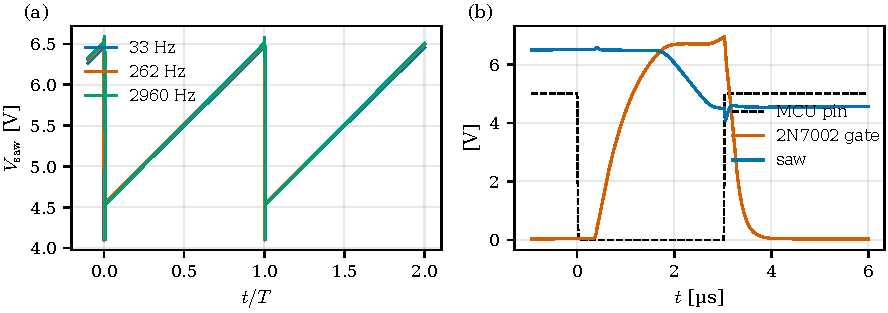
\includegraphics[width=\textwidth]{s1_dco_waveforms.pdf}
\caption{S1: (a) saw at \SI{33}{Hz}, \SI{262}{Hz} and \SI{2.96}{kHz} over two periods (time normalised to the period);
(b) reset detail at \SI{4.19}{kHz}: MCU pin, 2N7002 gate and saw.}\label{fig:s1a}
\end{figure}
\begin{figure}[ht]
\centering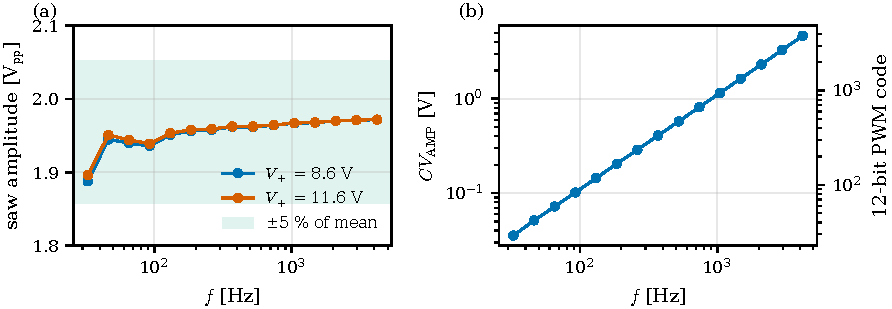
\includegraphics[width=\textwidth]{s1_dco_amplitude.pdf}
\caption{S1: (a) saw amplitude versus note at both supply corners; (b) firmware CV\sub{AMP} law and 12-bit code.}\label{fig:s1b}
\end{figure}

\subsection{S2 -- Control-voltage filters}
The first iteration used 12-bit PWM at \SI{11.7}{kHz}. It reached only \SI{-66.7}{dB} ripple and
\SI{2.2}{ms} settling. Switching to 10-bit PWM at \SI{46.9}{kHz} with 2-bit sigma-delta dithering keeps
12-bit resolution and moves the carrier up by a factor of four.

\begin{table}[h]
\centering\small
\caption{S2 results at the worst-case duty cycle (\SI{50}{\percent}), dither active.}\label{tab:s2}
\begin{tabular}{@{}l r r r r r@{}}
\toprule
Channel & Full scale & Ripple & re FS & Settling 1\,\% & Settling 0.1\,\% \\
\midrule
LIN & \SI{2.95}{V} & \SI{271}{\micro V_{pp}} & \SI{-81}{dB} & \SI{1.31}{ms} & \SI{1.88}{ms} \\
EXP & \SI{187}{mV} & \SI{12}{\micro V_{pp}} & \SI{-84}{dB} & \SI{1.22}{ms} & \SI{1.68}{ms} \\
\bottomrule
\end{tabular}
\end{table}
The EXP ripple corresponds to 0.8\,cent of cutoff modulation.

\begin{figure}[ht]
\centering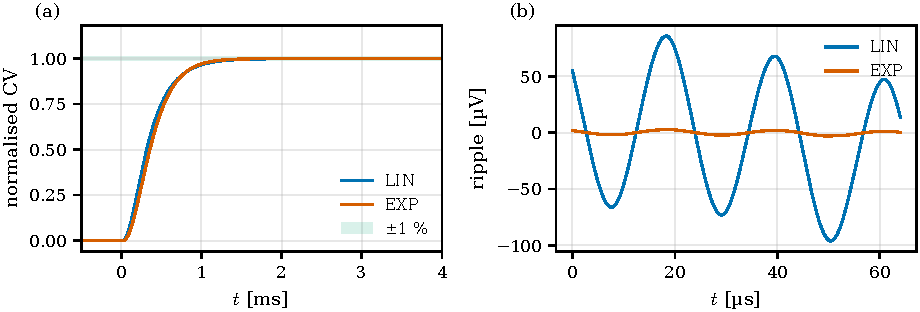
\includegraphics[width=\textwidth]{s2_cv_filter.pdf}
\caption{S2: (a) normalised \SIrange{10}{90}{\percent} step response; (b) steady-state ripple at \SI{50}{\percent} duty with dither.}\label{fig:s2}
\end{figure}

\subsection{S3 -- Ladder filter}
\begin{table}[h]
\centering\small
\caption{S3 results.}\label{tab:s3}
\begin{tabular}{@{}l l@{}}
\toprule
Quantity & Value \\
\midrule
\SI{-3}{dB} cutoff range (CV\sub{CUT} 0--5\,V) & \SIrange{19.9}{19800}{Hz} ($\approx$ 10 octaves) \\
Tracking & 2.05\,oct/V, log-linear \\
Slope (one octave above cutoff) & \SI{-23.1}{dB/oct} \\
Passband gain (ladder in $\to$ INA out) & \SI{20.4}{dB}, flat within \SI{1.6}{dB} \\
Resonance peak at CV\sub{CUT} = 2.5\,V & 4.8 / 13.6 / 20.7 / 28.9\,dB at CV\sub{RES} = 1 / 2 / 2.5 / 2.8\,V \\
Self-oscillation threshold & CV\sub{RES} $\approx$ \SI{3.1}{V}; \SIrange{0.11}{0.29}{V_{pp}} (soft-limited) \\
Supply sensitivity & +19\,cent between \SI{9}{V} and \SI{12}{V} input \\
Temperature drift & $-13.4$\,cent/K (accepted, see Section~\ref{sec:open}) \\
\bottomrule
\end{tabular}
\end{table}
\begin{figure}[ht]
\centering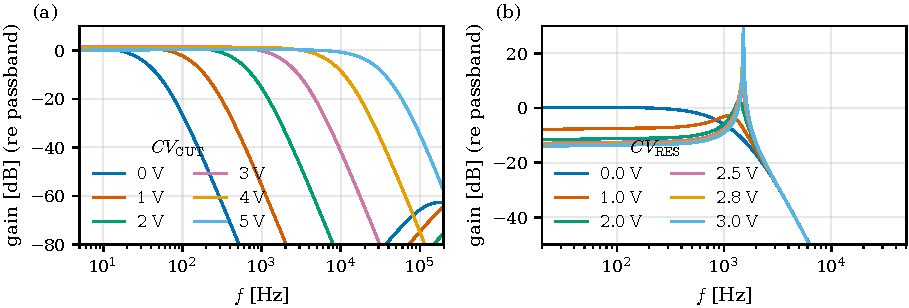
\includegraphics[width=\textwidth]{s3_vcf_response.pdf}
\caption{S3: (a) filter response for CV\sub{CUT} = 0--5\,V without resonance; (b) response at CV\sub{CUT} = \SI{2.5}{V}
for CV\sub{RES} below the self-oscillation threshold.}\label{fig:s3a}
\end{figure}
\begin{figure}[ht]
\centering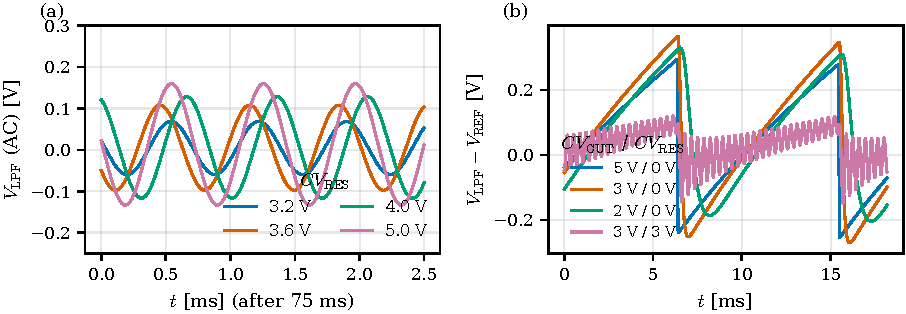
\includegraphics[width=\textwidth]{s3_vcf_transient.pdf}
\caption{S3: (a) steady-state self-oscillation for several CV\sub{RES} above threshold; (b) \SI{110}{Hz} saw through
the filter at different cutoff and resonance settings.}\label{fig:s3b}
\end{figure}

\subsection{S4 -- VCA}
\begin{itemize}
  \item \textbf{Gain}: maximum \SI{+7.4}{dB}. THD is 0.06 / 0.21 / 0.81\,\% at 0.3 / 0.6 /
    \SI{1.2}{V_{pp}} input.
  \item \textbf{Off attenuation}: \SI{121}{dB}. Without the \SI{470}{k\ohm} anti-offset resistor a
    \SI{+7}{mV} LM324 offset would leave only \SI{52}{dB}.
  \item \textbf{Feed-through}: with realistic mismatch (\SI{\pm1}{\percent} collector resistors,
    \SIrange{1}{2}{mV} $V_\mathrm{BE}$ offset) the CV feed-through is 94--\SI{101}{mV} per note, an audible
    thump. Both error terms scale with the tail current, so one static offset trim cancels both. After the
    two-point calibration the residual is \SI{0.58}{mV} and \SI{0.08}{mV} in the two mismatch cases.
\end{itemize}
\begin{figure}[ht]
\centering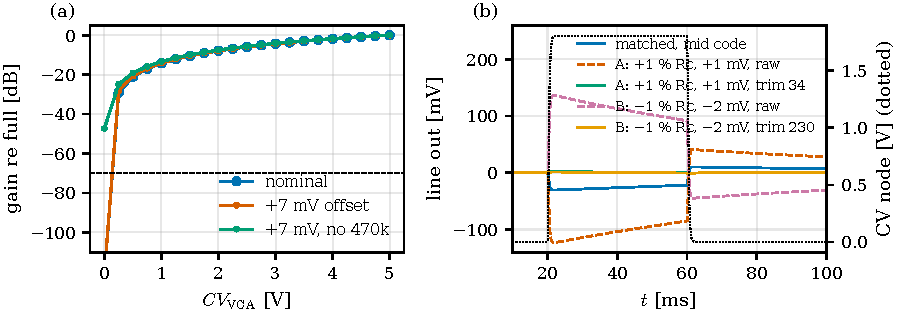
\includegraphics[width=\textwidth]{s4_vca.pdf}
\caption{S4: (a) gain versus CV\sub{VCA} (nominal, with \SI{+7}{mV} op-amp offset, and without the anti-offset resistor);
(b) CV feed-through for a 0 $\to$ full-scale step without signal, before and after the trim calibration.}\label{fig:s4}
\end{figure}

\subsection{S5 -- Touch sensing}
\begin{itemize}
  \item \textbf{Model}: the ch32fun slope method. The pin is released to the internal pull-down, and the
    ADC sample-and-hold samples the first \SI{0.625}{\micro s} of the decay. The model includes the
    multiplexer (\SI{30}{pF} common capacitance, \SI{470}{\ohm} on-resistance), the trace and the pad.
  \item \textbf{Sensitivity}: the multiplexer costs about a factor of five in sensitivity compared with a
    direct pin, but the margin stays large. A \SI{5}{pF} touch gives 14.8--20.8\,LSB per sample (V003) or
    57--81\,LSB (V002). The worst-case SNR is 39 and 152 with 16 samples per pad.
  \item \textbf{Scan rate}: a full scan takes \SI{0.69}{ms} (\SI{1.4}{kHz}).
\end{itemize}
\begin{figure}[ht]
\centering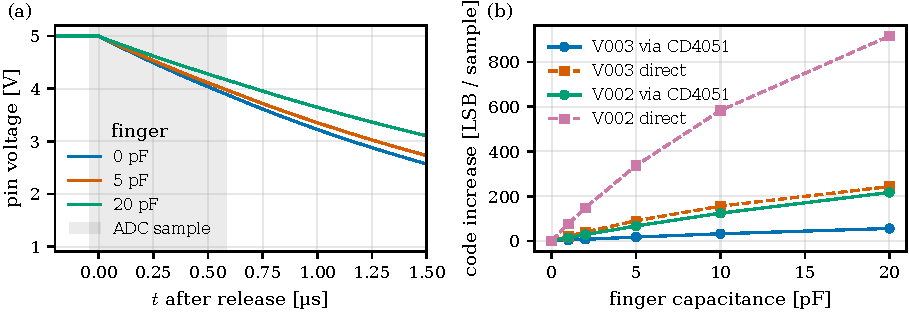
\includegraphics[width=\textwidth]{s5_touch.pdf}
\caption{S5: (a) pin voltage after release for 0, 5 and \SI{20}{pF} finger capacitance; (b) ADC code increase per
sample versus finger capacitance, through the multiplexer and direct.}\label{fig:s5}
\end{figure}

\subsection{S6 -- Complete voice}
The complete analog circuit was simulated with the firmware behaviour modelled in Python:
\begin{itemize}
  \item quantised timer periods,
  \item a sub-oscillator toggled once per period,
  \item a pulse-width LFO,
  \item ADSR envelopes,
  \item all CVs mapped through the calibrations of S1, S3 and S4.
\end{itemize}
The score is an eight-note bass line with filter envelope, followed by a held note with a slow resonant
sweep. The line output peaks at \SI{1.22}{V_{pp}}. The loopback node stays within
\SIrange{2.34}{2.88}{V}, well inside the ADC range.
\begin{figure}[ht]
\centering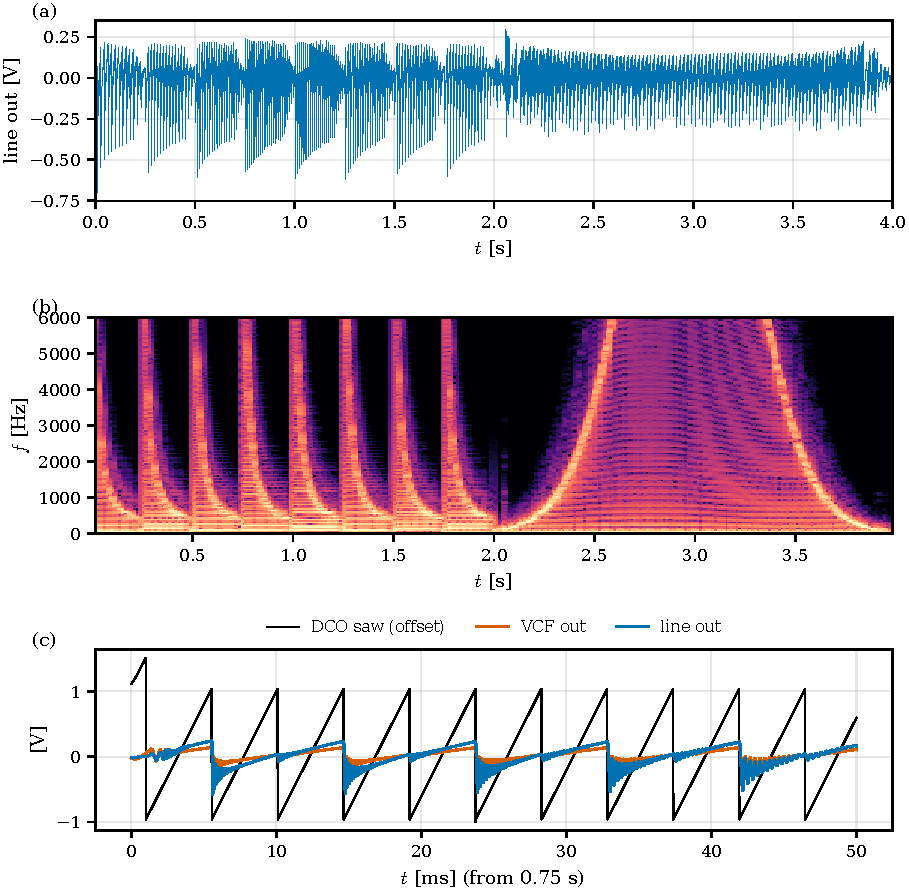
\includegraphics[width=\textwidth]{s6_voice.pdf}
\caption{S6: (a) line out; (b) spectrogram; (c) detail at \SI{0.75}{s}: DCO saw, filter output and line out.}\label{fig:s6}
\end{figure}

\subsection{S7 -- Power and references}
\begin{itemize}
  \item \textbf{Ripple}: with \SI{200}{mV_{pp}} of \SI{100}{Hz} ripple on the input, the line-output hum
    is \SI{-81}{dB} relative to \SI{1.33}{V_{pp}} at both \SI{9}{V} and \SI{12}{V}.
  \item \textbf{Current}: 31 and \SI{32}{mA} at 9 and \SI{12}{V}, including an assumed \SI{15}{mA} for the MCU, logic
    and LEDs. (Revision 0.1 of this report gave 33 and \SI{42}{mA} from two model errors that partly
    cancelled: the 78L05 model drew only its quiescent current from the input, and the TL072 macromodel drew
    about \SI{4}{mA} per amplifier instead of \SI{1.4}{mA}. Both were found at bring-up,
    Section~\ref{sec:vv}; the corrected model matches the measured \SI{25}{mA} of board 1 within
    \SI{1}{mA}.)
  \item \textbf{VREF buffer history}: the first VREF buffer (TL072 driving \SI{10}{\micro F} through
    \SI{100}{\ohm} outside the loop) let \SI{1.1}{mV_{pp}} of hum through, \SI{-47}{dB} at the output. A
    dual-loop variant fixed the hum but had a \SI{48}{\ohm} impedance peak. The final plain follower with
    an RC snubber has \SI{5}{m\ohm} at \SI{100}{Hz} and a single well-damped peak.
  \item \textbf{Power-on pop}: about \SI{3}{V}, decaying in about \SI{0.3}{s}. It is accepted: switch the
    synth on before the amplifier.
\end{itemize}
\begin{figure}[ht]
\centering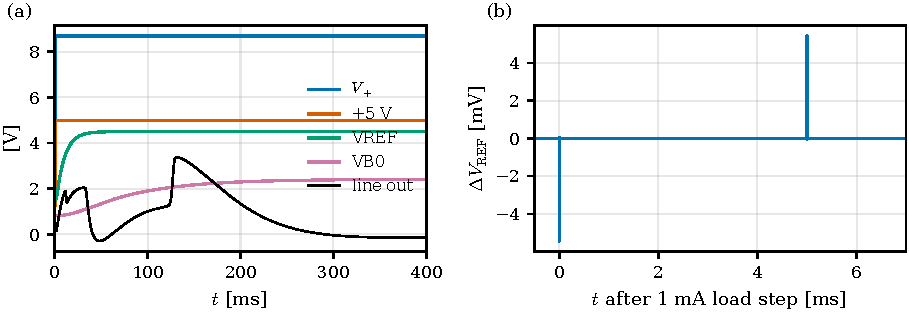
\includegraphics[width=\textwidth]{s7_power.pdf}
\caption{S7: (a) power-up at \SI{9}{V}; (b) VREF response to a \SI{1}{mA} load step.}\label{fig:s7}
\end{figure}

\subsection{S8 -- Pulse output as PWM DAC}\label{sec:s8}
S8 (\file{sim/s8\_dac/}) checks the DAC mode of Section~\ref{sec:kettle} on the real netlist from the pulse
input through mixer, ladder, VCA and line out, with the DCO held in reset. A \SI{1}{kHz} test tone at
\SI{-3}{dBFS} is encoded exactly as the firmware does it: \SI{15.625}{kHz} samples, 8-bit duty with
first-order error feedback. Three PWM variants are compared with an ideal DAC of the same scale, a continuous
source that interpolates linearly between the samples (Table~\ref{tab:s8}):
\begin{itemize}
  \item \textbf{edge, hold}: TIM2 counting up at \SI{187.5}{kHz}, each sample held for 12 periods (the first
    firmware version);
  \item \textbf{centre, hold}: TIM2 counting up and down at \SI{93.75}{kHz}, so the pulses are centred in
    the period; each sample held for 6 periods;
  \item \textbf{centre, interpolated}: in addition, the duty is interpolated linearly from the previous
    sample over the 6 periods (the firmware).
\end{itemize}
Results:
\begin{itemize}
  \item \textbf{Second harmonic}: with edge-aligned PWM the pulse centre moves with the duty, so the signal
    also modulates the pulse position. That adds a second harmonic at \SI{-45}{dB} (\SI{0.6}{\percent}).
    Centred pulses remove it: \SI{-68}{dB}, as clean as the ideal DAC. The third harmonic comes from the ladder
    itself in all cases.
  \item \textbf{Images}: holding each sample leaves images at $f_s \pm f$, \SI{-26}{dB} at a \SI{20}{kHz}
    cutoff. Linear interpolation lowers them by \SI{23}{dB} to the level of the ideal DAC.
  \item \textbf{Carrier}: halving the carrier to \SI{93.75}{kHz} for the centred pulses leaves it
    \SI{28}{dB} below the tone with the filter fully open. It is ultrasonic and falls below \SI{-74}{dB} at
    cutoffs of \SI{5}{kHz} and lower (the kettle uses \SI{4}{kHz}).
  \item \textbf{Noise}: without the images, \SIrange{-52}{-56}{dB} in the audio band, about the board's own
    noise floor. The level matches the ideal DAC within \SI{0.4}{dB}.
\end{itemize}

\begin{table}[h]
\centering\small
\caption{S8: \SI{1}{kHz} at \SI{-3}{dBFS} through the pulse input, three PWM variants and an ideal DAC
(\file{docs/results/s8\_dac.csv}); levels relative to the \SI{1}{kHz} tone. The firmware uses
\emph{centre, interpolated}.}\label{tab:s8}
\setlength{\tabcolsep}{4.5pt}
\begin{tabular}{@{}l l r r r r r r@{}}
\toprule
Cutoff & Source & 1\,kHz [mV] & H2 [dB] & H3 [dB] & Image [dB] & Carrier [dB] & Noise [dB] \\
\midrule
\SI{20}{kHz} & edge, hold & 292 & $-45$ & $-47$ & $-26$ & $-53$ & $-43$ \\
 & centre, hold & 292 & $-68$ & $-47$ & $-27$ & $-28$ & $-50$ \\
 & centre, interpolated & 290 & $-69$ & $-47$ & $-49$ & $-28$ & $-52$ \\
 & ideal & 295 & $-66$ & $-55$ & $-50$ & -- & $-49$ \\
\midrule
\SI{5}{kHz} & edge, hold & 348 & $-46$ & $-42$ & $-43$ & $-87$ & $-55$ \\
 & centre, hold & 348 & $-66$ & $-42$ & $-43$ & $-74$ & $-56$ \\
 & centre, interpolated & 346 & $-67$ & $-42$ & $-66$ & $-74$ & $-56$ \\
 & ideal & 359 & $-65$ & $-43$ & $-67$ & -- & $-51$ \\
\bottomrule
\end{tabular}
\end{table}

\subsection{Design changes found by simulation}\label{sec:lesson}
Table~\ref{tab:changes} lists every change that the simulations caused. The most instructive was the
\emph{CV network loading} bug:
\begin{itemize}
  \item \textbf{The bug}: the last RC stage of each control-voltage filter was designed as a divider for an
    ideal source, but it sits behind the series resistance of the first two stages. The real LIN ratio was
    therefore 0.36 instead of 0.6, and the cutoff range shrank to \SIrange{44}{4000}{Hz}.
  \item \textbf{Why the block tests missed it}: the individual block simulations had driven the dividers
    with ideal voltages.
  \item \textbf{How it was found}: only when the behavioural model (Section~\ref{sec:behav}) could not
    match the full-voice simulation.
  \item \textbf{Fix}: all networks were redesigned with the loading included, and every simulation now
    drives the CVs through the real networks.
\end{itemize}

\begin{table}[h]
\centering\small
\caption{Design changes caused by the simulations.}\label{tab:changes}
\begin{tabularx}{\textwidth}{@{}l X X@{}}
\toprule
Block & Change & Reason \\
\midrule
DCO & \SI{2.2}{k\ohm} gate resistor & slower switch-off edge, smaller charge-injection spike \\
CV filters & 10-bit PWM at \SI{46.9}{kHz} + 2-bit $\Sigma\Delta$ dither & ripple $-67 \to -81$\,dB, settling $2.2 \to 1.3$\,ms \\
CV filters & load-aware networks & correct DC ratios \\
VCF & ladder capacitors 47 $\to$ \SI{33}{nF} & top of range above \SI{15}{kHz} \\
VCF & mixer to VB0 via \SI{10}{k\ohm} / \SI{1}{\micro F}, \SI{150}{k\ohm}/\SI{470}{k\ohm} sources & settling $0.44\,\mathrm{s} \to 15$\,ms \\
VCF & resonance VCA with difference amplifier, 1:13 input, \SI{22}{k\ohm} feedback & no volt-level DC steps into the ladder \\
VCA & \SI{470}{k\ohm} anti-offset resistor & off attenuation $52 \to 121$\,dB \\
VCA & bases from VREF, 8-bit R-2R trim DAC & feed-through $\approx 100 \to < 0.6$\,mV \\
VCA & $R_E$ 3 $\to$ \SI{4.7}{k\ohm} & maximum gain $+11 \to +7.4$\,dB (headroom) \\
System & audio loopback to PD5 & self-test and calibration without extra ICs \\
Power & VREF follower with \SI{10}{\ohm} + \SI{1}{\micro F} snubber & hum $-47 \to -81$\,dB, stable \\
\bottomrule
\end{tabularx}
\end{table}

% =====================================================================================================
\section{Behavioural model and audio}\label{sec:behav}
A fast Python/numba model of the voice (\file{sim/behav/}) renders audio in seconds instead of the minutes
ngspice needs. It mirrors the hardware split:
\begin{itemize}
  \item \textbf{Firmware layer}: patch parameters, envelopes, LFO, glide, accent and slide, timer
    quantisation, 12-bit CVs at \SI{1}{kHz}.
  \item \textbf{Analog layer} at \SI{192}{kHz}: band-limited oscillators (polyBLEP), the S2 filters, a
    tanh ladder, the VCA law and the output coupling.
\end{itemize}
The model's constants are taken from the ngspice results. The resonance loop gain was obtained by inverting
the S3 resonance peaks. Two parameters were fitted to the self-oscillation pitch and amplitude.

Compared with ngspice on the S6 score, the model matches:
\begin{itemize}
  \item the level within \SI{-0.6}{dB} (\SI{1.1}{dB} rms),
  \item the self-oscillation pitch within \SI{2}{\percent} and its amplitude within \SI{7}{\percent},
  \item the overall brightness (spectral centroid) within 300\,cent; the difference is concentrated where
    the resonance sits exactly at threshold.
\end{itemize}
It renders 19 feature clips and three demo tunes in the firmware step format (3 bytes per step): an original
acid line, Bach's Prelude in C and Beethoven's \emph{Ode to Joy}. The audio files are in
\file{docs/audio/features/}.

\begin{figure}[ht]
\centering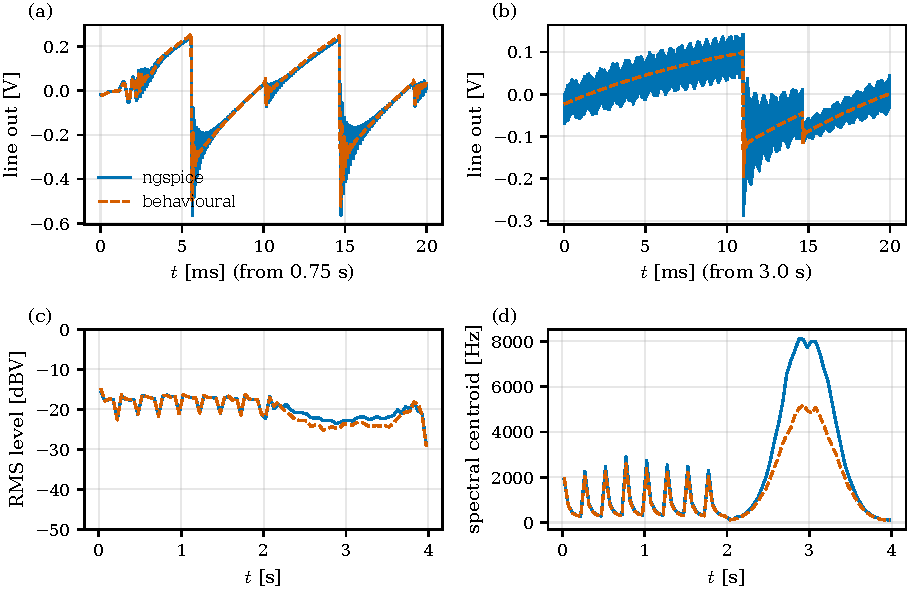
\includegraphics[width=\textwidth]{behav_validation.pdf}
\caption{Behavioural model versus ngspice on the S6 score: (a, b) waveform details, (c) RMS level, (d) spectral centroid.}\label{fig:behav}
\end{figure}

\begin{figure}[ht]
\centering
\begin{subfigure}{0.49\textwidth}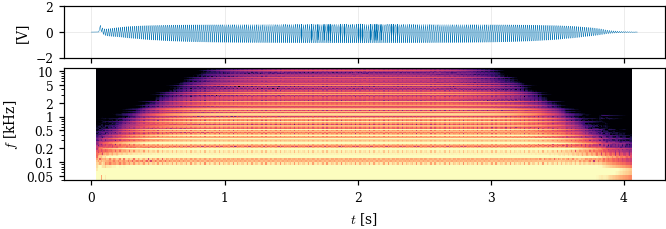
\includegraphics[width=\linewidth]{audio/08_cutoff.png}\caption{cutoff sweep}\end{subfigure}\hfill
\begin{subfigure}{0.49\textwidth}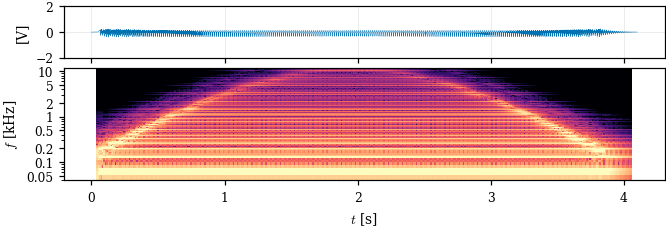
\includegraphics[width=\linewidth]{audio/10_res_sweep.png}\caption{resonance sweep}\end{subfigure}\\[4pt]
\begin{subfigure}{0.49\textwidth}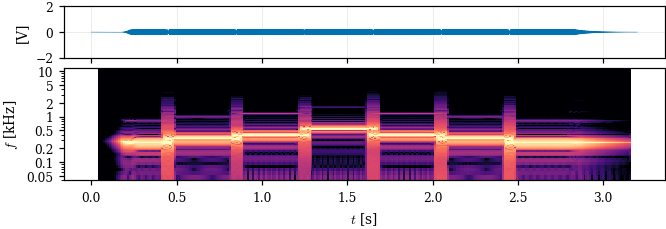
\includegraphics[width=\linewidth]{audio/11_self_osc.png}\caption{self-oscillation}\end{subfigure}\hfill
\begin{subfigure}{0.49\textwidth}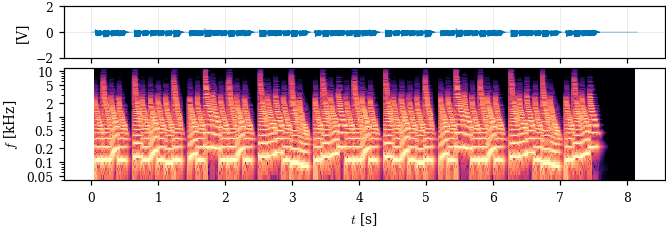
\includegraphics[width=\linewidth]{audio/tune_acid.png}\caption{demo tune (acid line)}\end{subfigure}
\caption{Spectrograms of selected behavioural-model clips.}\label{fig:audio}
\end{figure}

% =====================================================================================================
\section{PCB design}\label{sec:pcb}

\subsection{Board and stack-up}
The board is \SI{100}{mm}\,$\times$\,\SI{100}{mm}, \SI{1.6}{mm}, four layers, with all components on the
top side (Table~\ref{tab:stack}). A first two-layer attempt was abandoned:
\begin{itemize}
  \item it could not be routed completely,
  \item ground islands between dense traces left pads without a reliable ground,
  \item some touch lines ran under other keys.
\end{itemize}
The four-layer stack solves all three problems. It also gives the analog audio path a continuous ground
reference, at little extra cost.

\begin{table}[h]
\centering\small
\caption{Layer stack.}\label{tab:stack}
\begin{tabularx}{\textwidth}{@{}l X@{}}
\toprule
Layer & Use \\
\midrule
F.Cu & components, signals, GND pour; no tracks across the keyboard \\
In1.Cu & solid GND plane \\
In2.Cu & split power plane: VP under the analog area, +5\,V under the MCU column and the keys I/O row, GND under the keyboard \\
B.Cu & signals, GND pour; below each key only that key's own line \\
\bottomrule
\end{tabularx}
\end{table}

\paragraph{Touch pads.} On the standard JLCPCB stack-up, the first inner layer lies only about
\SI{0.2}{mm} below the pads. A plane there would dominate the pad capacitance and ruin the touch
sensitivity. The pads are therefore protected on the other three layers:
\begin{itemize}
  \item both inner layers have a copper cut-out under every pad,
  \item the bottom layer has a pour-free keep-out under every pad, open only in a small strip at the top of
    the pad where the key's own via and trace arrive,
  \item on the top layer, the pads have a \SI{1}{mm} local clearance.
\end{itemize}

\subsection{Floorplan}
Figure~\ref{fig:floor} shows the floorplan:
\begin{itemize}
  \item \textbf{Analog area} (top left): the blocks in signal-flow order, from power and references
    through the oscillator, ladder, output amplifier and resonance to the VCA and the CV filters.
  \item \textbf{Right-hand column}: MIDI input (not populated), the trim DAC directly next to the VCA, and
    the MCU.
  \item \textbf{Keys I/O row}: the two multiplexers and the two LED shift registers sit in a full-width row
    directly above the LEDs and keys. Each chip is above the keys it serves, so the 32 LED and touch lines
    are short vertical drops instead of long buses across the board.
\end{itemize}
Moving these chips there from a column on the right made the board routable.

\begin{figure}[ht]
\centering
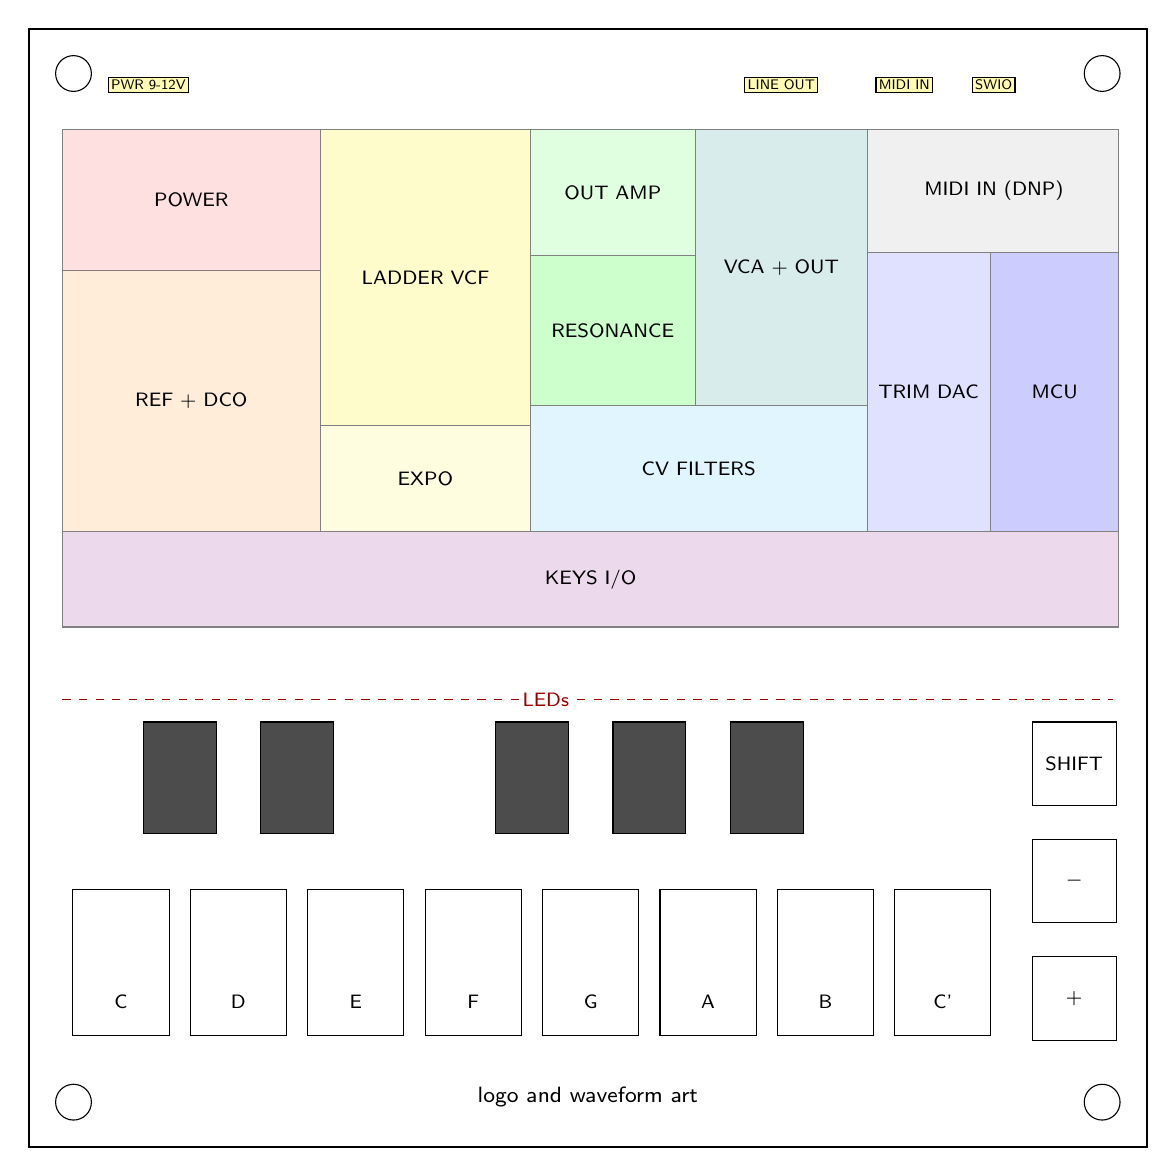
\begin{tikzpicture}[x=0.142cm,y=-0.142cm,font=\scriptsize\sffamily]
\draw[thick] (0,0) rectangle (100,100);
\filldraw[fill=red!12,draw=black!50] (3.00,9.00) rectangle (26.08,21.58);
\node[align=center,text width=2.95cm] at (14.54,15.29) {POWER};
\filldraw[fill=orange!15,draw=black!50] (3.00,21.58) rectangle (26.08,45.00);
\node[align=center,text width=2.95cm] at (14.54,33.29) {REF + DCO};
\filldraw[fill=yellow!20,draw=black!50] (26.08,9.00) rectangle (44.85,35.46);
\node[align=center,text width=2.40cm] at (35.46,22.23) {LADDER VCF};
\filldraw[fill=yellow!12,draw=black!50] (26.08,35.46) rectangle (44.85,45.00);
\node[align=center,text width=2.40cm] at (35.46,40.23) {EXPO};
\filldraw[fill=green!12,draw=black!50] (44.85,9.00) rectangle (59.62,20.28);
\node[align=center,text width=1.89cm] at (52.23,14.64) {OUT AMP};
\filldraw[fill=green!20,draw=black!50] (44.85,20.28) rectangle (59.62,33.72);
\node[align=center,text width=1.89cm] at (52.23,27.00) {RESONANCE};
\filldraw[fill=teal!15,draw=black!50] (59.62,9.00) rectangle (75.00,33.72);
\node[align=center,text width=1.97cm] at (67.31,21.36) {VCA + OUT};
\filldraw[fill=cyan!12,draw=black!50] (44.85,33.72) rectangle (75.00,45.00);
\node[align=center,text width=3.85cm] at (59.92,39.36) {CV FILTERS};
\filldraw[fill=gray!12,draw=black!50] (75.00,9.00) rectangle (97.50,20.00);
\node[align=center,text width=2.88cm] at (86.25,14.50) {MIDI IN (DNP)};
\filldraw[fill=blue!12,draw=black!50] (75.00,20.00) rectangle (86.00,45.00);
\node[align=center,text width=1.41cm] at (80.50,32.50) {TRIM DAC};
\filldraw[fill=blue!20,draw=black!50] (86.00,20.00) rectangle (97.50,45.00);
\node[align=center,text width=1.47cm] at (91.75,32.50) {MCU};
\filldraw[fill=violet!15,draw=black!50] (3.00,45.00) rectangle (97.50,53.50);
\node[align=center,text width=12.08cm] at (50.25,49.25) {KEYS I/O};
\draw[fill=white] (3.95,77) rectangle (12.55,90);
\node at (8.25,87) {C};
\draw[fill=white] (14.45,77) rectangle (23.05,90);
\node at (18.75,87) {D};
\draw[fill=white] (24.95,77) rectangle (33.55,90);
\node at (29.25,87) {E};
\draw[fill=white] (35.45,77) rectangle (44.05,90);
\node at (39.75,87) {F};
\draw[fill=white] (45.95,77) rectangle (54.55,90);
\node at (50.25,87) {G};
\draw[fill=white] (56.45,77) rectangle (65.05,90);
\node at (60.75,87) {A};
\draw[fill=white] (66.95,77) rectangle (75.55,90);
\node at (71.25,87) {B};
\draw[fill=white] (77.45,77) rectangle (86.05,90);
\node at (81.75,87) {C'};
\draw[fill=black!70] (10.25,62.00) rectangle (16.75,72.00);
\draw[fill=black!70] (20.75,62.00) rectangle (27.25,72.00);
\draw[fill=black!70] (41.75,62.00) rectangle (48.25,72.00);
\draw[fill=black!70] (52.25,62.00) rectangle (58.75,72.00);
\draw[fill=black!70] (62.75,62.00) rectangle (69.25,72.00);
\draw[fill=white] (89.75,62.00) rectangle (97.25,69.50);
\node at (93.50,65.75) {SHIFT};
\draw[fill=white] (89.75,72.47) rectangle (97.25,79.97);
\node at (93.50,76.22) {$-$};
\draw[fill=white] (89.75,82.95) rectangle (97.25,90.45);
\node at (93.50,86.70) {$+$};
\draw[dashed,red!60!black] (3,60.0) -- (97,60.0) node[pos=0.46,fill=white,inner sep=1pt] {LEDs};
\draw (4.0,4.0) circle (1.6);
\draw (96.0,4.0) circle (1.6);
\draw (4.0,96.0) circle (1.6);
\draw (96.0,96.0) circle (1.6);
\node[draw,fill=yellow!30,inner sep=1pt] at (10.7,5.0) {\tiny PWR 9-12V};
\node[draw,fill=yellow!30,inner sep=1pt] at (67.3,5.0) {\tiny LINE OUT};
\node[draw,fill=yellow!30,inner sep=1pt] at (78.3,5.0) {\tiny MIDI IN};
\node[draw,fill=yellow!30,inner sep=1pt] at (86.3,5.0) {\tiny SWIO};
\node[font=\footnotesize\sffamily] at (50,95.5) {logo and waveform art};
\end{tikzpicture}

\caption{Floorplan (generated from \file{hw/pcb\_place.py}). Connectors along the top edge; the scope
ground pins and test points are not shown.}
\label{fig:floor}
\end{figure}

\subsection{Placement}
Placement is scripted (\file{hw/pcb\_place.py}, \file{hw/gen\_pcb.py}):
\begin{itemize}
  \item \textbf{Anchors}: ICs, the ladder transistor column, connectors, keys and LEDs have explicit
    positions.
  \item \textbf{Greedy placement}: every other part is placed greedily inside its block, most-connected
    parts first. Each goes to the free spot that minimises the distance to the pads it connects to, with
    \SI{0.3}{mm} spacing to leave routing channels.
  \item \textbf{Decoupling capacitors}: they are placed at their IC's supply pin.
  \item \textbf{Test points}: each goes into the block holding most pins of its net, with its net name
    printed next to it. VCAOUT and XCUT\_IN did not fit and sit on the free top edge.
  \item \textbf{Scope ground}: two through-hole \SI{2.54}{mm} pins on the top edge.
\end{itemize}

\subsection{Routing}
Routing is automated in several stages (\file{gen\_pcb.py --route}):
\begin{enumerate}
  \item \textbf{Plane stitching}: every GND, VP and +5\,V pad gets a short track to its own via into its
    plane. The vias are locked so that the autorouter keeps them.
  \item \textbf{Pre-routing}: the few supply pins outside their plane region are routed on the still empty
    board with an A* grid router (\file{hw/pcb\_maze.py}) and locked.
  \item \textbf{Autorouting}: Freerouting 1.9 does two passes. The inner layers are declared as power
    planes, so signals stay on the outer layers.
  \item \textbf{Ground grid}: GND stitching vias go on a \SI{2.5}{mm} grid wherever both outer pours are
    filled. They keep clear of the mounting holes and of all silkscreen artwork.
  \item \textbf{Island check}: GND islands are detected by a connectivity analysis and bridged if
    necessary (\file{hw/pcb\_gnd.py}).
  \item \textbf{Leftovers}: the A* maze router finishes any remaining connection. A rip-up mode
    (\file{--repair}) exists for stubborn cases.
\end{enumerate}
The final board has \SI{0.25}{mm} tracks (\SI{0.3}{mm} for stitching), \SI{0.2}{mm} clearance and
\SI{0.6}{mm}/\SI{0.3}{mm} vias, all within JLCPCB's standard capabilities. It has 246 footprints,
1773 track segments (\SI{2.5}{m} on F.Cu, \SI{1.9}{m} on B.Cu) and 626 vias.

The KiCad design-rule check reports \textbf{0 violations, 0 unconnected pads and 0 schematic-parity errors}.

\begin{figure}[p]
\centering
\begin{subfigure}{0.49\textwidth}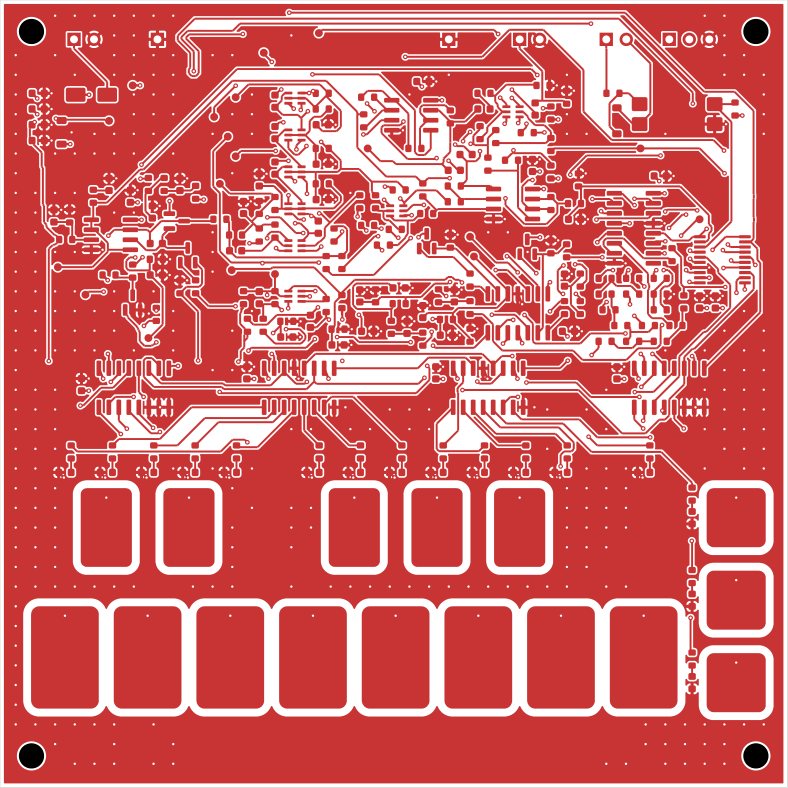
\includegraphics[width=\linewidth]{pcb/layer_F.png}\caption{F.Cu}\end{subfigure}\hfill
\begin{subfigure}{0.49\textwidth}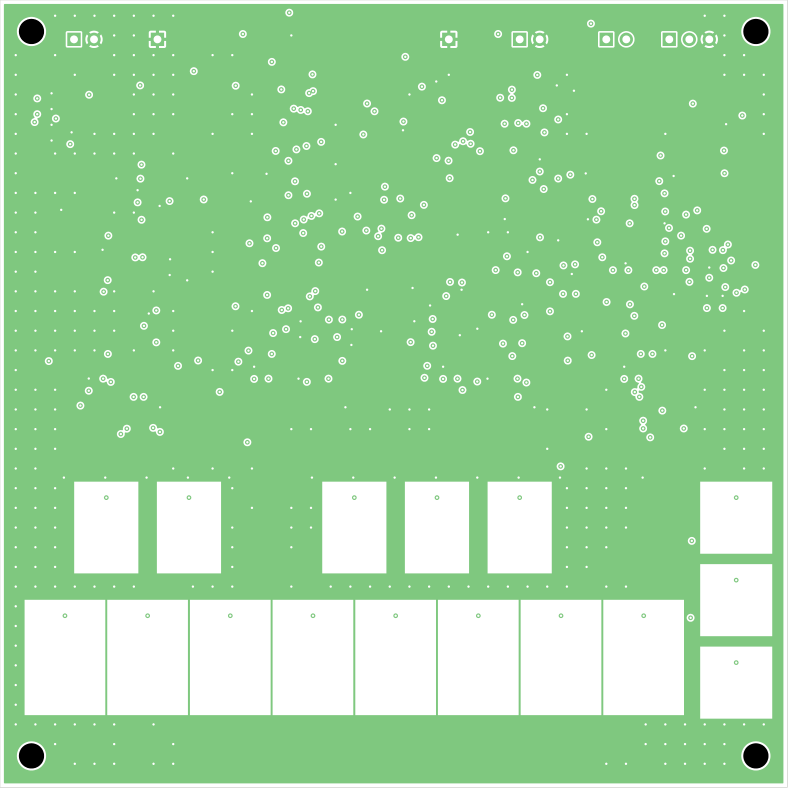
\includegraphics[width=\linewidth]{pcb/layer_In1.png}\caption{In1.Cu (GND)}\end{subfigure}\\[6pt]
\begin{subfigure}{0.49\textwidth}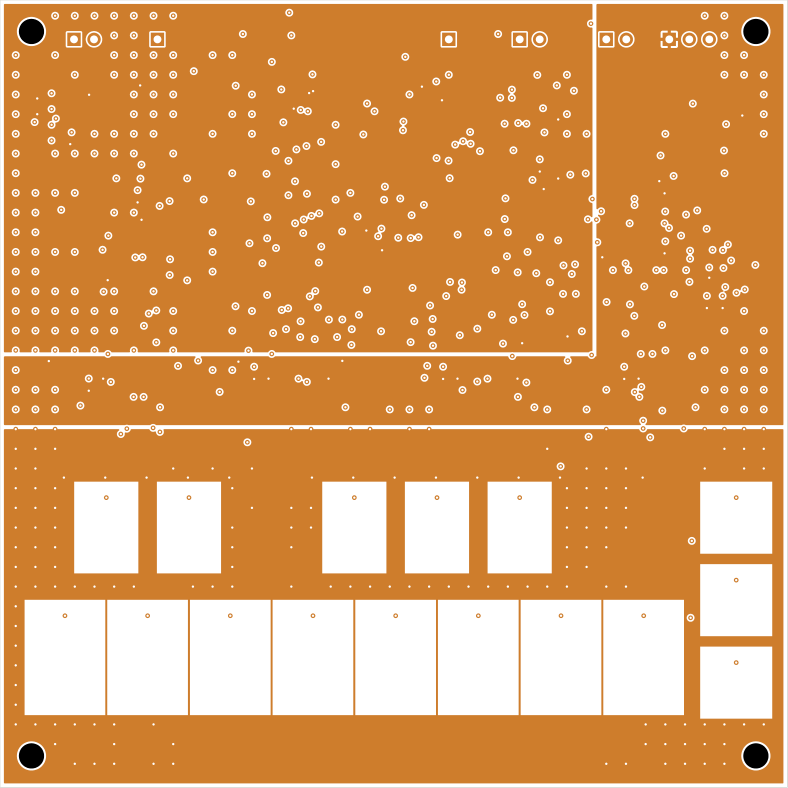
\includegraphics[width=\linewidth]{pcb/layer_In2.png}\caption{In2.Cu (VP / +5\,V / GND)}\end{subfigure}\hfill
\begin{subfigure}{0.49\textwidth}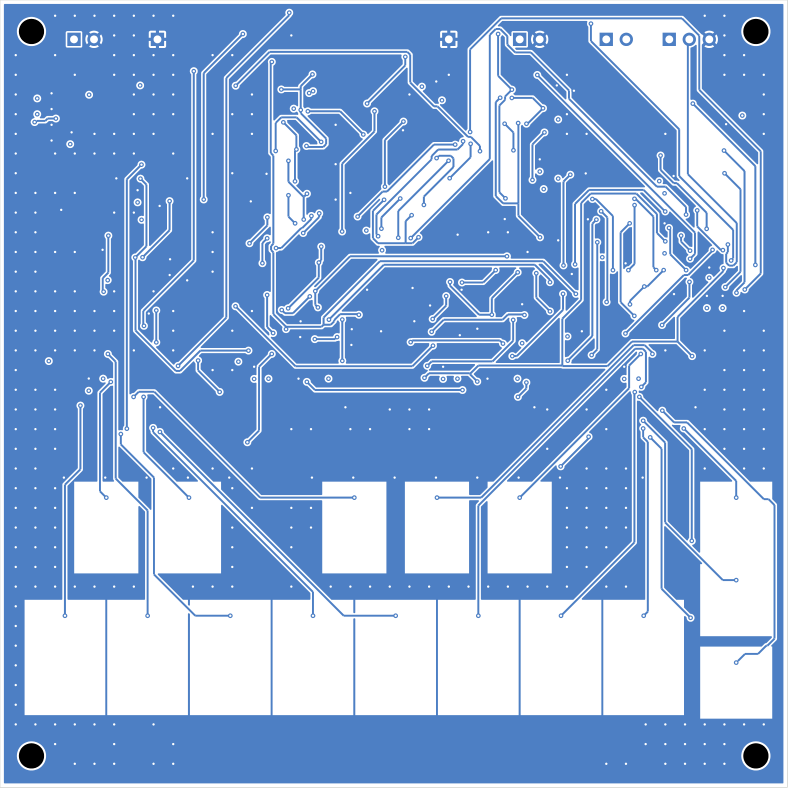
\includegraphics[width=\linewidth]{pcb/layer_B.png}\caption{B.Cu}\end{subfigure}
\caption{Copper layers (seen from the top).}\label{fig:layers}
\end{figure}

\subsection{Silkscreen}
The silkscreen documents the design on the board itself:
\begin{itemize}
  \item a dashed frame with a title for every functional block,
  \item a piano-style keybed with hatched black keys,
  \item a strip with the logo, a resonant sawtooth and the ladder response family,
  \item on the back, the signal-flow diagram and the credits.
\end{itemize}
All silkscreen text is at least \SI{0.8}{mm} high with \SI{0.15}{mm} lines, JLCPCB's minimum.

\begin{figure}[ht]
\centering
\begin{subfigure}{0.49\textwidth}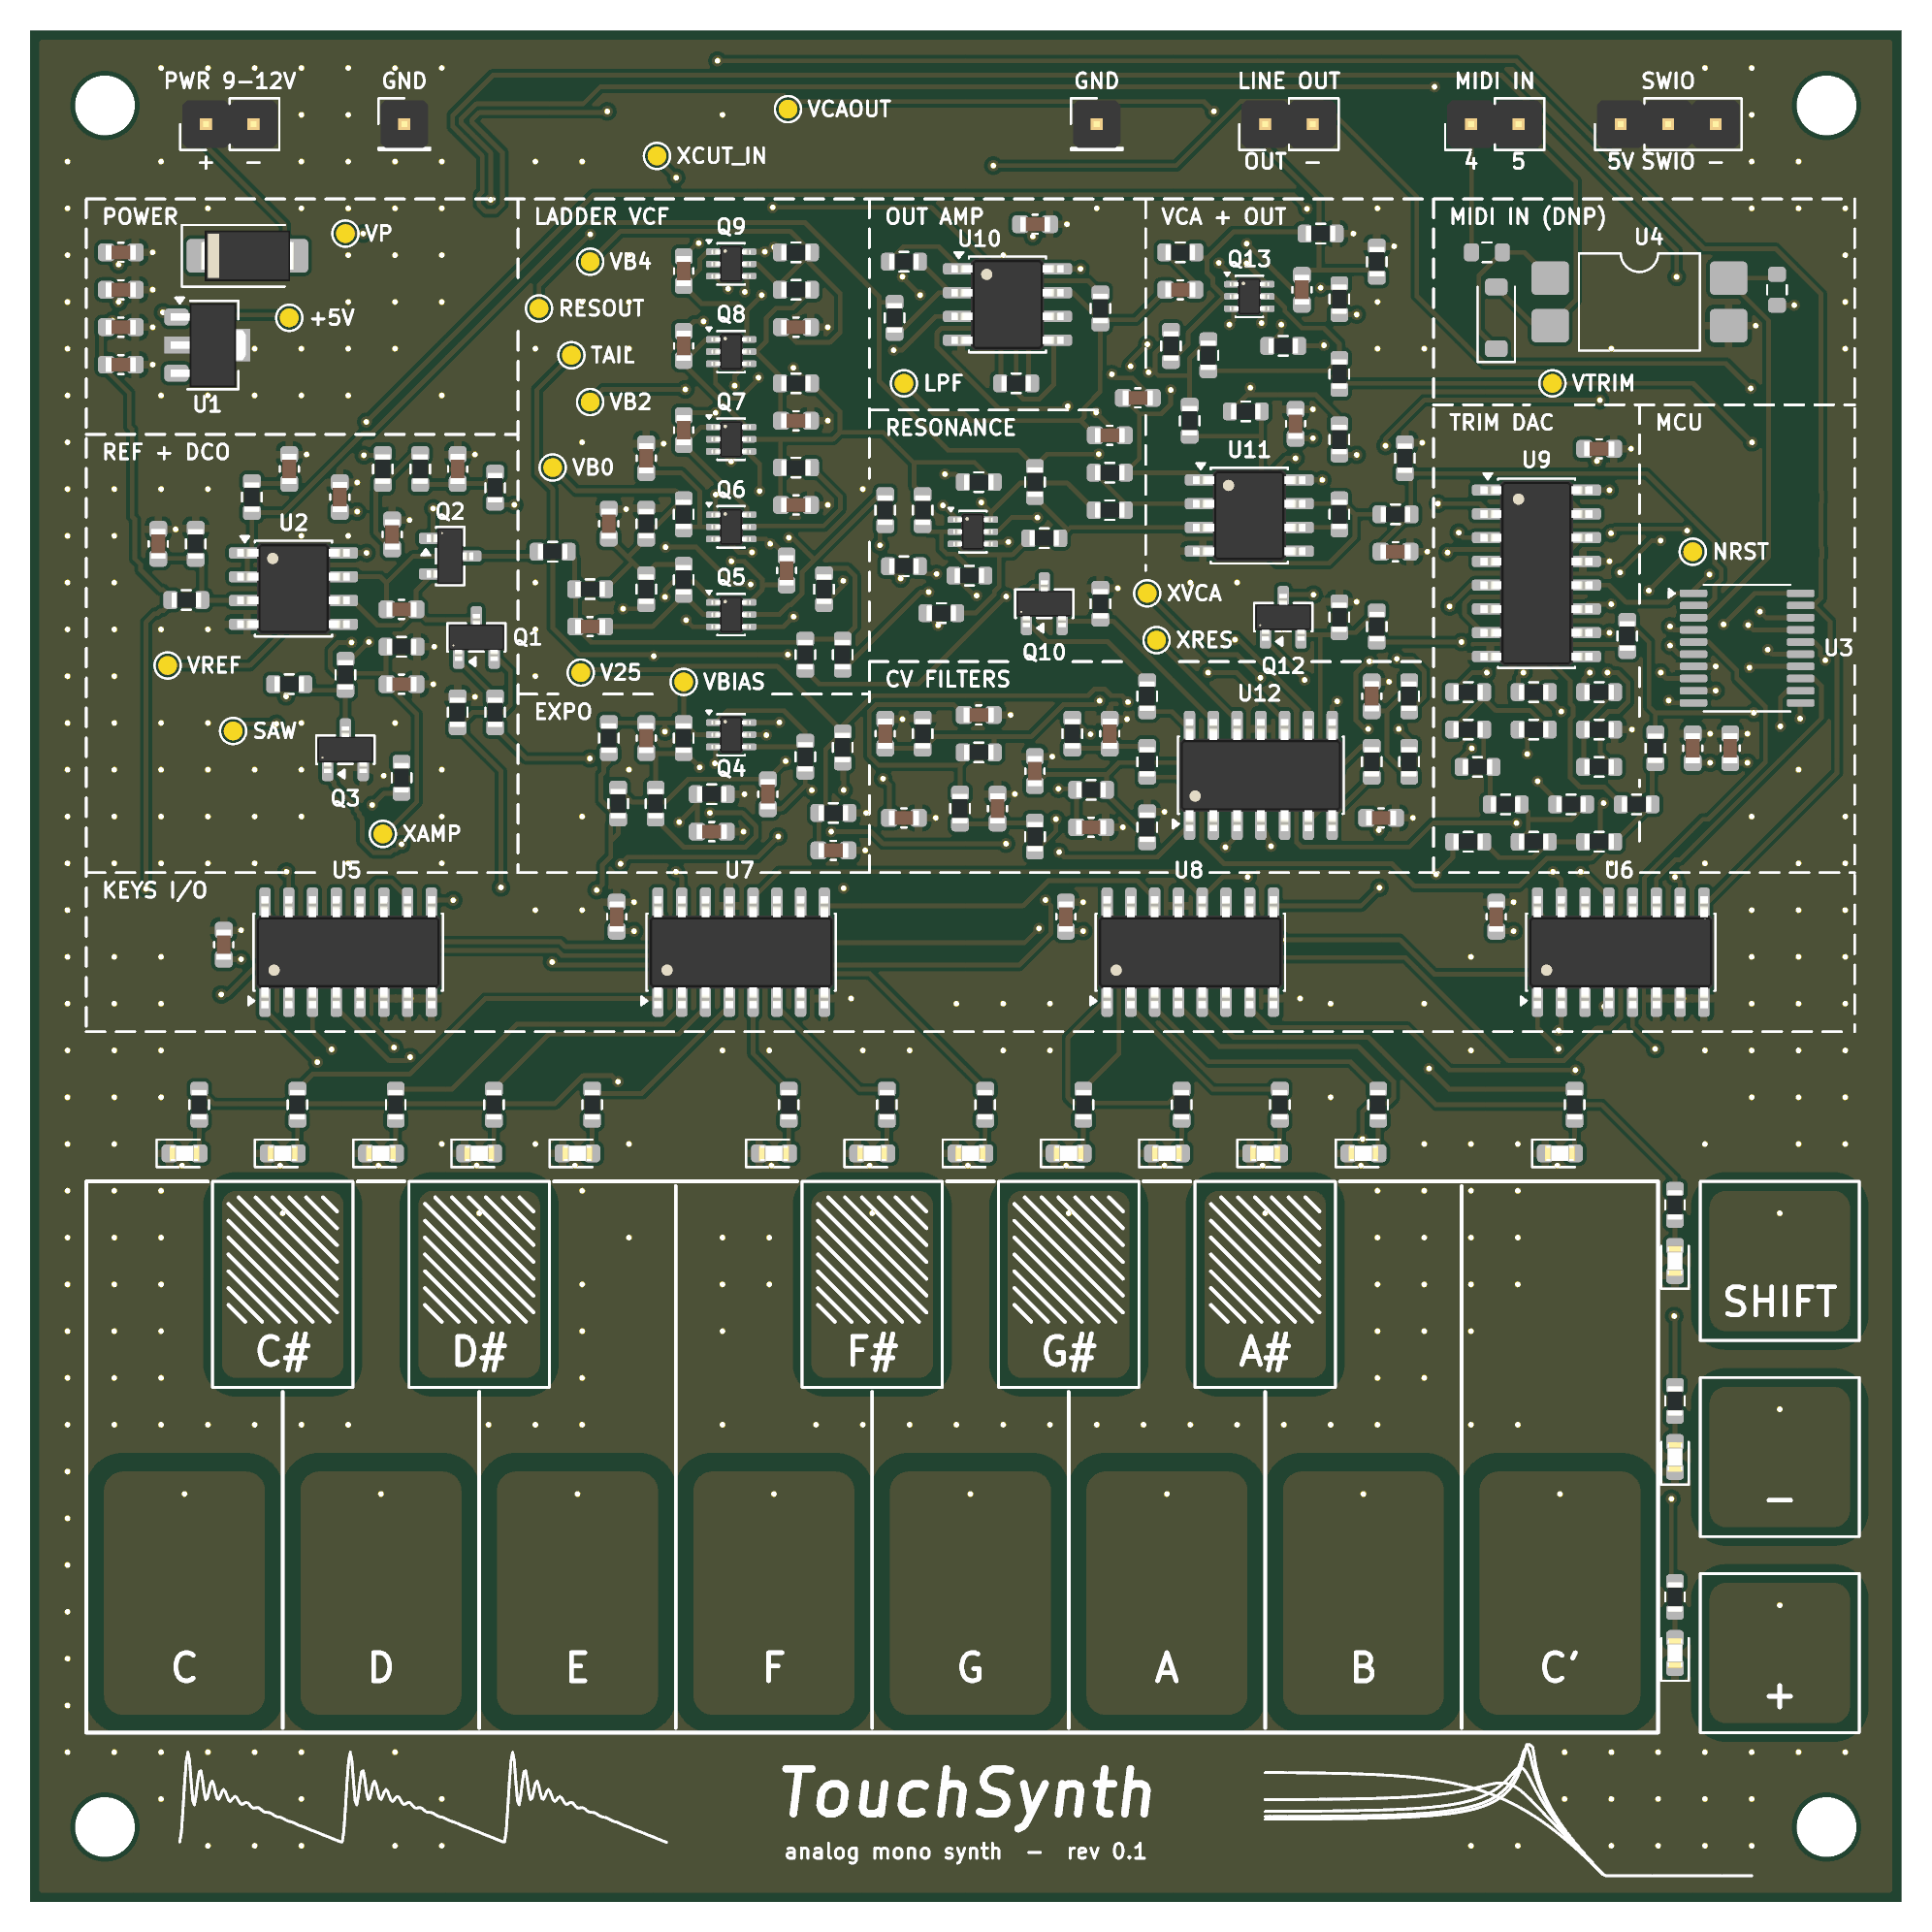
\includegraphics[width=\linewidth]{pcb/render_top.png}\caption{top}\end{subfigure}\hfill
\begin{subfigure}{0.49\textwidth}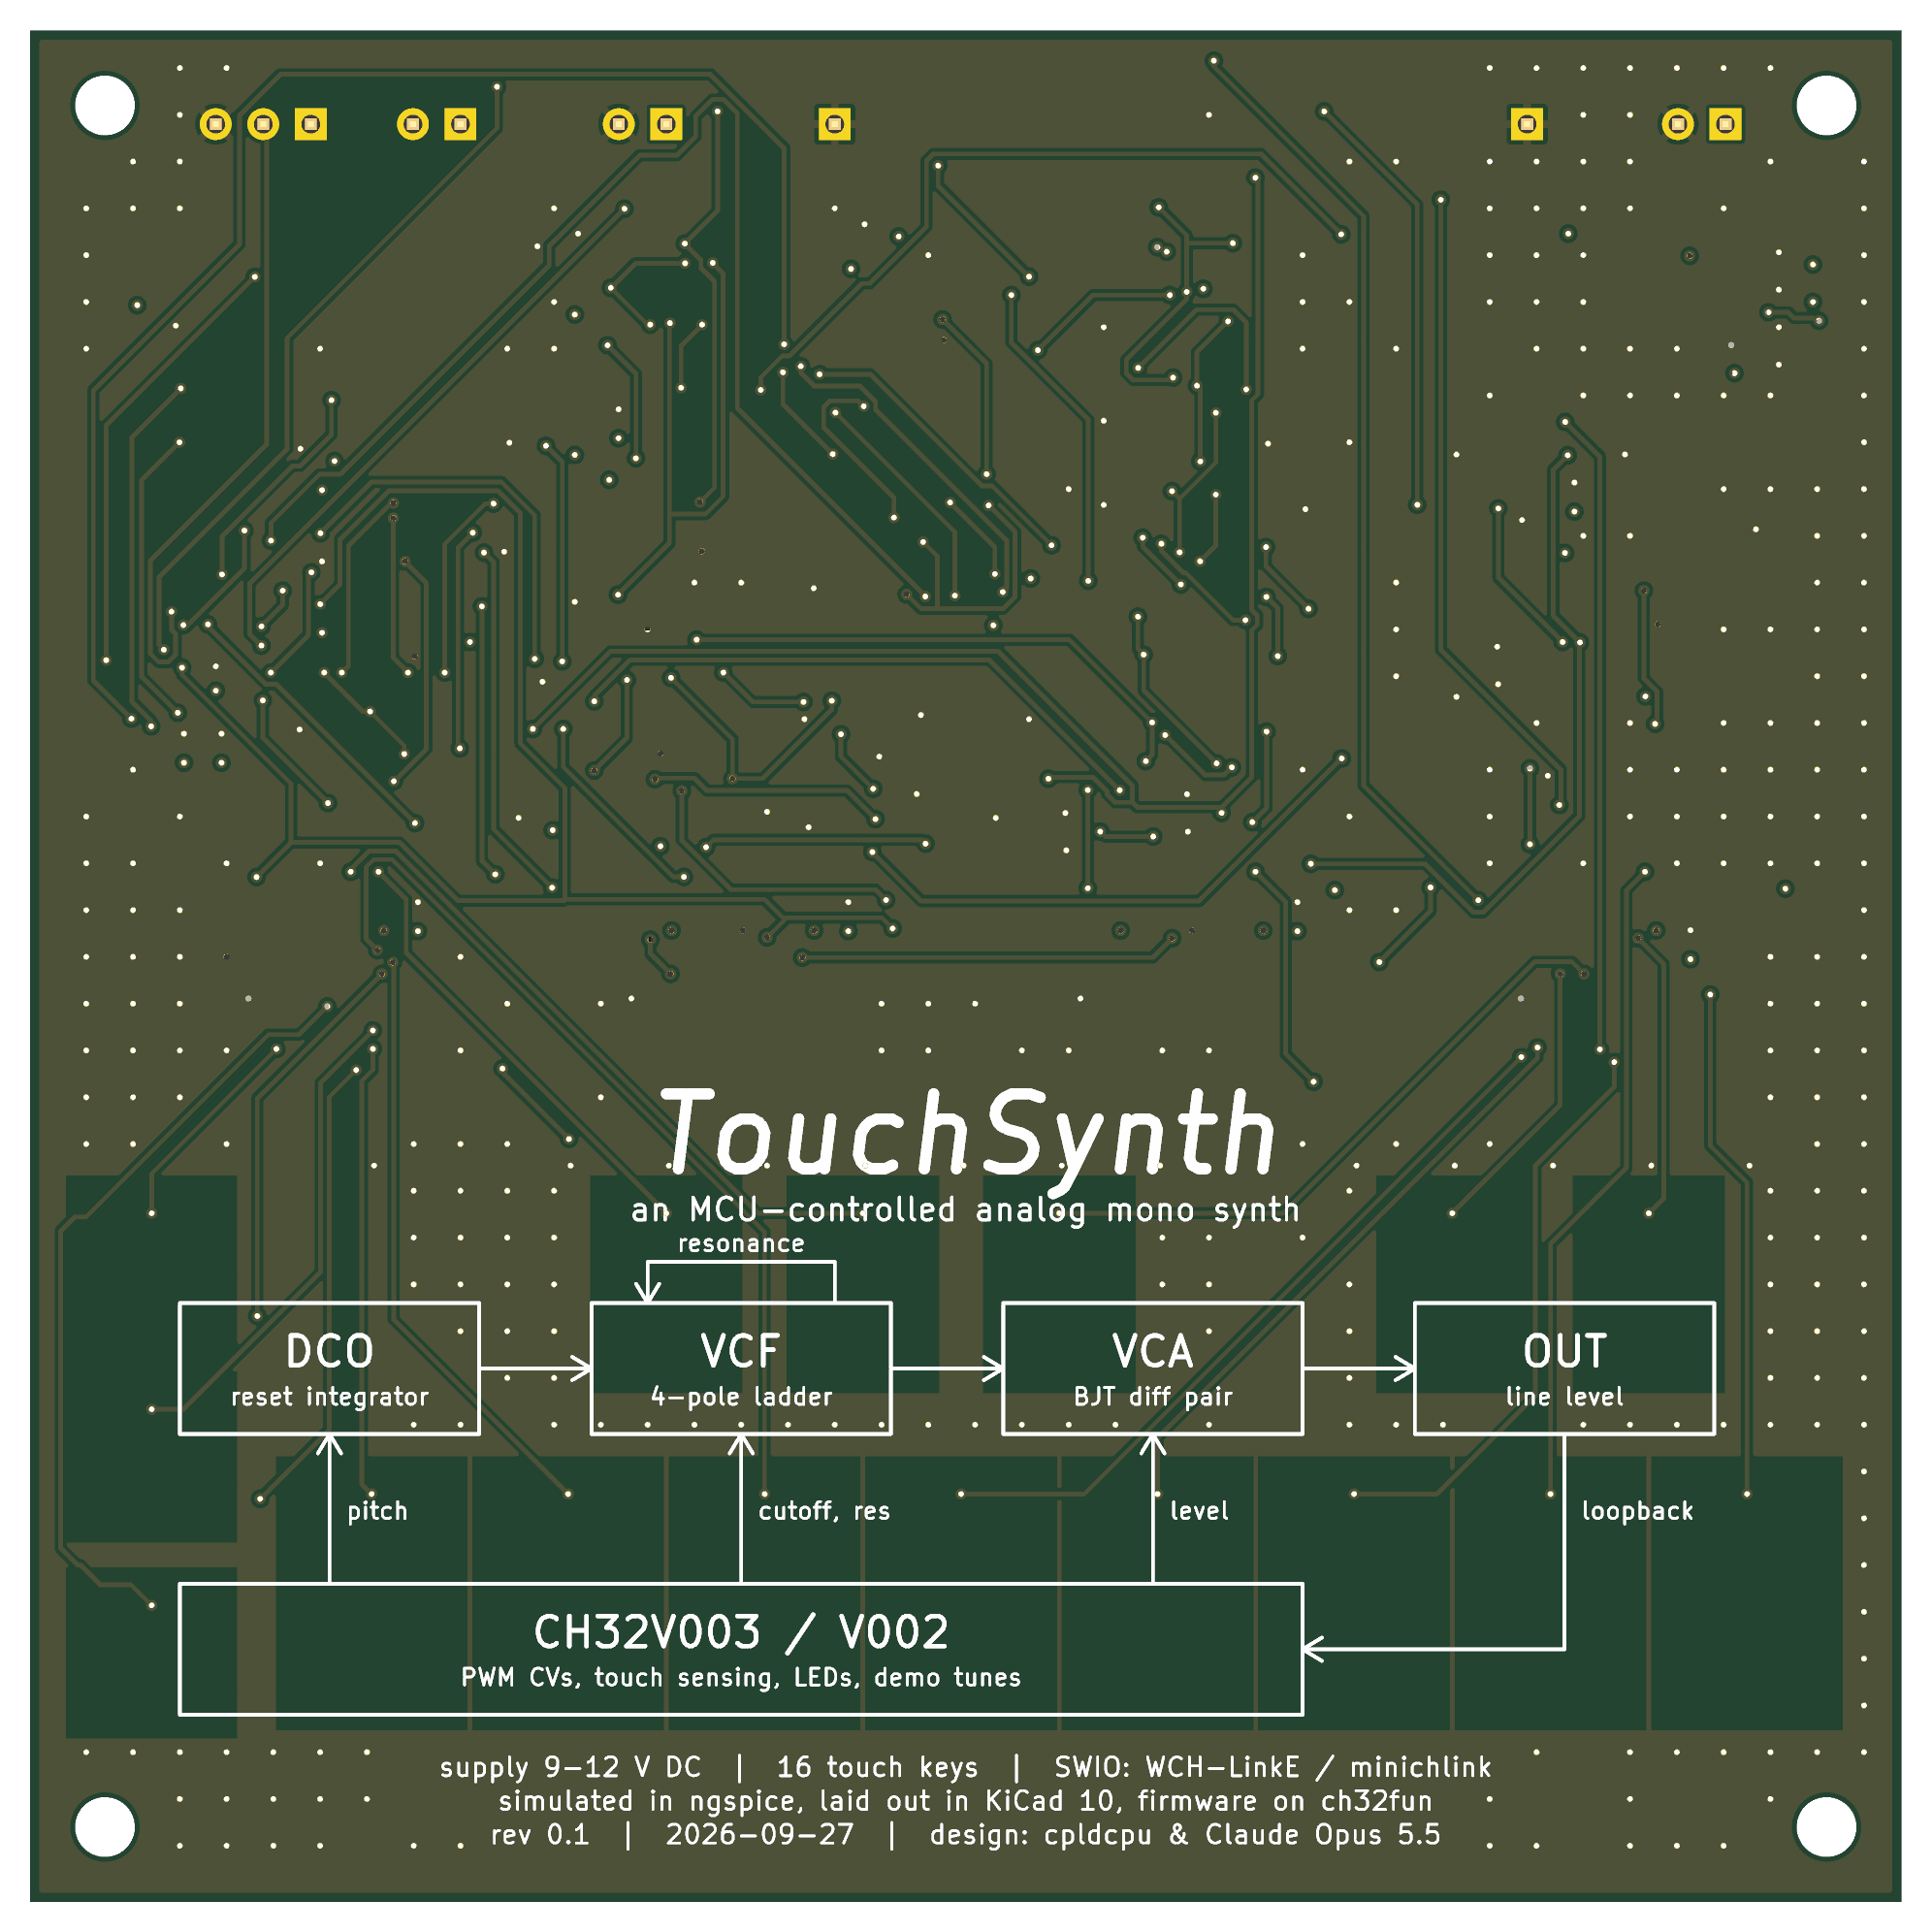
\includegraphics[width=\linewidth]{pcb/render_bottom.png}\caption{bottom}\end{subfigure}
\caption{Rendered board.}\label{fig:renders}
\end{figure}

\subsection{Fabrication data}
\file{hw/fab.py} writes the JLCPCB outputs:
\begin{itemize}
  \item the Gerber files of all four copper layers plus mask, paste, silkscreen and outline, and the
    Excellon drill file;
  \item the BOM;
  \item the placement (CPL) file, with rotation offsets for the SOT, SOIC and TSSOP packages.
\end{itemize}
The MCU, the headers, the test points, the touch pads and the MIDI parts are excluded from assembly.

% =====================================================================================================
\section{Bill of materials}\label{sec:bom}
JLCPCB assembles \statPlaced\ parts in \statBomlines\ BOM lines: \statBasiclines\ Basic and
\statPromolines\ Promotional Extended (BC847BS, CD4051). The components cost about
USD~\statPartscost\ per board at list price, excluding PCB, assembly fees and the MCU (Table~\ref{tab:bom}).
The design has \statParts\ parts in total; \statDnp\ are marked do-not-populate (the MCU and the MIDI input).

{\small\begin{longtable}{@{}l r l l l r p{5.2cm}@{}}
\caption{Assembled parts (JLCPCB PCBA, top side). Unit prices from the JLCPCB parts list at the time of design.}\label{tab:bom}\\
\toprule Value & Qty & Package & LCSC & Library & USD/pc & Designators\\ \midrule\endfirsthead
\toprule Value & Qty & Package & LCSC & Library & USD/pc & Designators\\ \midrule\endhead
\bottomrule\endfoot
4.7k & 29 & 0603 & C23162 & Basic & 0.0028 & {\footnotesize R16--R31, R49, R50, R56, R58, R75, R76, R83, R84, R91, R92, R95, R102, R103}\\
10k & 17 & 0603 & C25804 & Basic & 0.0018 & {\footnotesize R6, R7, R55, R63, R64, R66, R67, R73, R81, R82, R85--R88, R104, R106, R109}\\
1k & 15 & 0603 & C21190 & Basic & 0.0026 & {\footnotesize R1, R9--R12, R48, R52, R57, R62, R74, R78, R90, R94, R98, R99}\\
100k & 10 & 0603 & C25803 & Basic & 0.0031 & {\footnotesize R34, R36, R38, R40, R42, R44, R46, R65, R68, R108}\\
200k & 9 & 0603 & C25811 & Basic & 0.0023 & {\footnotesize R32, R33, R35, R37, R39, R41, R43, R45, R47}\\
15k & 4 & 0603 & C22809 & Basic & 0.0029 & {\footnotesize R51, R77, R93, R110}\\
470k & 4 & 0603 & C23178 & Basic & 0.0030 & {\footnotesize R70--R72, R96}\\
33k & 3 & 0603 & C4216 & Basic & 0.0022 & {\footnotesize R53, R59, R97}\\
22k & 3 & 0603 & C31850 & Basic & 0.0041 & {\footnotesize R89, R105, R107}\\
1.5k & 2 & 0603 & C22843 & Basic & 0.0019 & {\footnotesize R5, R60}\\
2.2k & 2 & 0603 & C4190 & Basic & 0.0018 & {\footnotesize R8, R54}\\
1M & 1 & 0603 & C22935 & Basic & 0.0019 & {\footnotesize R100}\\
2M & 1 & 0603 & C22976 & Basic & 0.0025 & {\footnotesize R101}\\
2.4k & 1 & 0603 & C22940 & Basic & 0.0026 & {\footnotesize R13}\\
9.1k & 1 & 0603 & C23260 & Basic & 0.0031 & {\footnotesize R2}\\
10 & 1 & 0603 & C22859 & Basic & 0.0032 & {\footnotesize R3}\\
3.3k & 1 & 0603 & C22978 & Basic & 0.0026 & {\footnotesize R4}\\
300k & 1 & 0603 & C23024 & Basic & 0.0054 & {\footnotesize R61}\\
150k & 1 & 0603 & C22807 & Basic & 0.0044 & {\footnotesize R69}\\
6.2k & 1 & 0603 & C4260 & Basic & 0.0023 & {\footnotesize R79}\\
120k & 1 & 0603 & C25808 & Basic & 0.0015 & {\footnotesize R80}\\
100n & 17 & 0603 & C14663 & Basic & 0.0122 & {\footnotesize C2, C4, C6, C15, C17--C22, C26, C28, C34, C36, C41, C45, C48}\\
33n & 8 & 0603 & C21117 & Basic & 0.0106 & {\footnotesize C23, C27, C30--C33, C37, C42}\\
1\textmu{} & 8 & 0603 & C15849 & Basic & 0.0752 & {\footnotesize C3, C7--C9, C16, C35, C39, C44}\\
10\textmu{} & 5 & 0603 & C96446 & Basic & 0.0541 & {\footnotesize C1, C10--C13}\\
22n & 3 & 0603 & C21122 & Basic & 0.0083 & {\footnotesize C24, C38, C43}\\
10\textmu{} & 3 & 0603 & C19702 & Basic & 0.0319 & {\footnotesize C5, C14, C46}\\
1n & 2 & 0603 & C1588 & Basic & 0.0089 & {\footnotesize C29, C47}\\
10n & 1 & 0603 & C57112 & Basic & 0.0108 & {\footnotesize C25}\\
4.7\textmu{} & 1 & 0603 & C19666 & Basic & 0.0294 & {\footnotesize C40}\\
red & 16 & 0603 & C2286 & Basic & 0.0075 & {\footnotesize D3--D18}\\
SS14 & 1 & D & C2480 & Basic & 0.0191 & {\footnotesize D1}\\
BC847BS & 8 & SOT-363 & C41375126 & Promo & 0.0281 & {\footnotesize Q4--Q9, Q11, Q13}\\
MMBT3904 & 4 & SOT-23 & C20526 & Basic & 0.0115 & {\footnotesize Q1, Q3, Q10, Q12}\\
2N7002 & 1 & SOT-23 & C8545 & Basic & 0.0178 & {\footnotesize Q2}\\
TL072 & 3 & SOIC-8 & C6961 & Basic & 0.1613 & {\footnotesize U2, U10, U11}\\
74HC595 & 3 & SOIC-16 & C5947 & Basic & 0.1152 & {\footnotesize U7--U9}\\
CD4051B & 2 & SOIC-16 & C21379 & Promo & 0.2574 & {\footnotesize U5, U6}\\
78L05 & 1 & SOT-89-3 & C71136 & Basic & 0.0892 & {\footnotesize U1}\\
LM324 & 1 & SOIC-14 & C71035 & Basic & 0.1658 & {\footnotesize U12}\\
\midrule
\multicolumn{2}{@{}l}{196 parts} & \multicolumn{3}{l}{40 BOM lines} & 3.65 & per board (parts only)\\
\end{longtable}
}

Hand-soldered (not in the assembly BOM):
\begin{itemize}
  \item the MCU (CH32V003F4P6 or CH32V002F4P6),
  \item the pin headers: power, line out, SWIO, MIDI and the two scope-ground pins,
  \item optionally the MIDI parts (LTV-817S, 1N4148W, \SI{220}{\ohm} and \SI{470}{\ohm}).
\end{itemize}

% =====================================================================================================
\section{Firmware}
Firmware version 0.1 (\file{firmware/touchsynth/}) is built on ch32fun for the CH32V003, CH32V002 and
CH32V006 from one code base. With the three demo tunes it uses 14.1\,KB of the 16\,KB flash of the smallest
part. The CH32V006 build (44.4\,KB) also holds the multitrack parts of Section~\ref{sec:tunes} and the
digital voice on the PWM DAC (Section~\ref{sec:kettle}). It runs on board 1 (Section~\ref{sec:board1}).
Its structure follows the timing of the design:
\begin{itemize}
  \item \textbf{TIM1 update interrupt} at \SI{46.875}{kHz}: loads the four CV compare registers with 2-bit
    sigma-delta dither (10-bit PWM, 12-bit effective) and clocks the noise LFSR. An interrupt was chosen over
    DMA bursts for simplicity; it costs a few percent of the CPU.
  \item \textbf{TIM2}: the DCO period. Channel 1 produces the \SI{3}{\micro s} active-low reset pulse,
    channel 2 the pulse wave, and the update interrupt toggles the sub-oscillator. In DAC mode (CH32V006
    only) TIM2 instead counts up and down at a fixed \SI{93.75}{kHz} with the DCO held in reset, and DMA1
    channel~2 loads the channel-2 duty from a ring buffer on every update (Section~\ref{sec:kettle}).
  \item \textbf{Control loop} at \SI{1}{kHz} (SysTick): glide, LFO, envelopes, key tracking, the CV laws,
    the percussion pitch envelope and wave switch, and the tune player. It mirrors the firmware layer of the behavioural model. All maths is fixed
    point, because the CH32V003 has no multiplier.
  \item \textbf{Main loop}: the touch scan of all 16 pads through the multiplexers with per-pad baselines
    and thresholds, the SHIFT/$-$/$+$ user interface, the LED and trim-DAC shift registers, MIDI input, a
    test console over SWIO for the verification plan (Section~\ref{sec:vv}), and in DAC mode the DSP that
    refills the DAC ring buffer.
\end{itemize}
The calibration tables, presets and demo tunes are generated from the simulation results and
\file{tunes.py} by \file{gen\_tables.py}; nothing is copied by hand.

\paragraph{Pin assignment check.} Writing the firmware was also a check of the pin assignment.
\file{check\_pins.py} compares every pin constant in the firmware with:
\begin{itemize}
  \item the net in the design,
  \item the port in the KiCad symbol,
  \item the timer, USART and ADC function of that port on each chip family.
\end{itemize}
All 16 signal pins pass on both families. The check found one difference that the firmware must handle: the
timer remap \emph{codes} differ (Table~\ref{tab:remap}). The same remaps also route complementary outputs to
PC3, PC4 and PD1 (SWIO). The firmware never enables them.

\begin{table}[h]
\centering\small
\caption{Timer remaps used by the firmware.}\label{tab:remap}
\begin{tabular}{@{}l l l@{}}
\toprule
Function & CH32V003 & CH32V002 / V006 \\
\midrule
TIM1 CH1--CH4 $\to$ PC6, PC7, PC0, PD3 & \texttt{TIM1\_REMAP} = 01 & \texttt{TIM1\_RM} = 0010 \\
TIM2 CH1, CH2 $\to$ PC5, PC2 & \texttt{TIM2\_REMAP} = 01 & \texttt{TIM2\_RM} = 010 \\
\bottomrule
\end{tabular}
\end{table}

% =====================================================================================================
\section{Demo tunes and instruments}\label{sec:tunes}
\subsection{Tune format and player}
A tune is a step sequence in flash with three bytes per step: note, length and flags. The length counts steps
of a per-tune step time (a sixteenth note for most tunes, a \SI{20}{ms} grid for the Toccata), so one step
holds up to 255 steps. Each tune names a preset. The flags are:
\begin{itemize}
  \item \textbf{slide}: glide into the note without restarting the envelopes;
  \item \textbf{accent}: the preset's accent filter-envelope depth and level;
  \item \textbf{hold} and \textbf{tie}: no release at the end of the step, and continue the previous note.
    Together they split notes longer than 255 steps;
  \item \textbf{sync}: the VCA opens fully for \SI{4}{ms}, a marker for aligning multitrack recordings.
\end{itemize}
Steps with a note number of 128 or more are \emph{control steps}. They take no time and set the cutoff
(in 1/16 octave), the resonance, the filter-envelope depth, the waveform mask or the volume. A preceding ramp
step sets a glide time for the next cutoff and resonance targets, which the \SI{1}{kHz} loop interpolates.
All filter sweeps in the pieces are such ramps.

The tunes are written in Python (\file{sim/behav/tunes.py}, \file{pieces.py}) and converted by
\file{gen\_tables.py}. The behavioural model plays the same step data, including the control steps, so
every tune can be heard before it is flashed.

\subsection{Built-in demos}
All builds hold three demos, cycled with SHIFT + C$'$:
\begin{itemize}
  \item \textbf{acid}: an original acid line (\SI{19}{s}, preset \emph{acid});
  \item \textbf{prelude}: Bach's Prelude in C (\SI{48}{s}, preset \emph{arp});
  \item \textbf{ode}: Beethoven's \emph{Ode to Joy} (\SI{35}{s}, preset \emph{lead} with glide and
    vibrato).
\end{itemize}
Board 1 recordings of the three demos are in \file{docs/audio/hw\_board1/}.

\subsection{Multitrack pieces}
The CH32V006 build also holds 30 single-voice parts of four multitrack pieces (Table~\ref{tab:pieces}).
The synth is monophonic, so a piece is recorded one part at a time from the line out and mixed on the PC:
\begin{itemize}
  \item \textbf{Recording}: the console disables the touch keys (\texttt{keys 0}) and starts the part. The
    oscilloscope records a single shot of \SI{50}{M} points with 8-bit resolution, which
    \file{tools/scope.py} boxcar-decimates to \SI{100}{kS/s}. The averaging (oversampling) raises the
    resolution.
  \item \textbf{Alignment}: each part starts with a sync step. If a take was captured without its sync pulse
    (the scope triggers only after its pre-trigger memory is full), its envelope is cross-correlated with
    the model render of the same part instead.
  \item \textbf{Clock}: the RC oscillator differs by about \SI{0.1}{\percent} between takes. The clock of
    each take is fitted from its note onsets (residual 2--\SI{5}{ms} rms), and the take is resampled onto
    a common clock.
  \item \textbf{Mix} (\file{tools/mix\_parts.py}, \file{suite.py}): noise gate, pan, Haas widening on pads,
    ping-pong delay and convolution reverb.
\end{itemize}

\begin{table}[h]
\centering\small
\caption{Multitrack pieces. Audio in \file{docs/audio/demo/} and \file{docs/audio/pieces/}
(\texttt{\_hw}: board 1, \texttt{\_model}: behavioural model).}\label{tab:pieces}
\begin{tabularx}{\textwidth}{@{}l >{\raggedright\arraybackslash}X >{\raggedright\arraybackslash}X r@{}}
\toprule
Piece & Source & Parts (preset) & Length \\
\midrule
TouchSynth Demo & original, 118\,bpm, 69 bars & kick, snare, hat, bass (acid), arp, lead, pad (sweep) & 2:24 \\
Queen Mary's March & Purcell, Z\,860, WIMA edition for four trumpets; two passes with filter sweeps
  & 4 trumpets (brass), 16$'$ bass (pedal), timpani (kettle, PWM DAC) & 2:41 \\
Toccata, mm.\,1--30 & Bach, BWV\,565, MusicXML; mordents and trill written out, fermatas doubled
  & 8 manual tracks (organ), pedal & 2:02 \\
Aerosphere & original, in the style of 1970s space-synth music, 100\,bpm, 68 bars
  & wind, 2 pads (strings), sequence (seq), bass (pedal), lead (theremin), kick, hat & 2:53 \\
Suite & Aerosphere intro (wind, pads) dissolving into the Toccata & -- & 2:19 \\
\bottomrule
\end{tabularx}
\end{table}

The Toccata has up to nine simultaneous voices. They are allocated to the eight manual tracks by nearest
pitch, so each track plays a continuous line and no note is dropped. Purcell's score has no drum part; the
timpani on C and G (tonic and dominant) are an addition and follow the harmony bar by bar.

\subsection{Instruments}
Every instrument is a preset of the one voice (Table~\ref{tab:presets}): the waveform mask (saw, pulse,
sub-octave square, noise), cutoff with key tracking, filter-envelope depth, resonance (1 = self-oscillation
threshold), two ADSR envelopes, glide and an LFO on pitch or pulse width.
\begin{itemize}
  \item \textbf{Brass}: saw and pulse with a slow filter attack (\SI{60}{ms}), so each note opens from
    dark like a trumpet.
  \item \textbf{Organ, pedal}: organ is saw, pulse and sub with full sustain and fast attack and release.
    Pedal is a saw without the sub: on board 1 the sub-octave of low pedal notes (\SI{33}{Hz}) was heard as
    pumping.
  \item \textbf{Strings}: a slow pulse-width modulation (\SI{0.4}{Hz}) stands in for an ensemble, with
    slow attack and release.
  \item \textbf{Wind}: noise through the filter just below self-oscillation. Control-step ramps sweep it
    into pitched gusts.
  \item \textbf{Theremin}: a pulse wave with \SI{120}{ms} glide and \SI{5.5}{Hz} vibrato of 25\,cent.
  \item \textbf{Seq, acid, arp, lead, sweep}: classic subtractive patches; fast filter envelopes for the
    sequence and acid line, a slow filter swell for the pad.
\end{itemize}

\begin{table}[h]
\centering\footnotesize
\caption{Presets (\file{sim/behav/tunes.py}). Cutoff at C4, envelope depth in octaves, ADSR times in s;
$\to$: waveform after the wave switch.}\label{tab:presets}
\setlength{\tabcolsep}{3.5pt}
\begin{tabular}{@{}l l r r r r l l@{}}
\toprule
Preset & Waveforms & Cutoff [Hz] & Key tr. & Env. & Res. & Filter ADSR & Amp ADSR \\
\midrule
acid & saw & 170 & 0.3 & 3.2 & 0.80 & .002/.09/0/.04 & .002/.2/.7/.02 \\
arp & saw + pulse, PWM & 700 & 0.5 & 3.0 & 0.55 & .001/.12/.1/.1 & .002/.18/.4/.12 \\
lead & saw + sub, vibrato & 1400 & 0.6 & 1.5 & 0.35 & .01/.5/.4/.3 & .01/.4/.85/.25 \\
sweep & saw + sub & 180 & 0.3 & 4.2 & 0.70 & 1.6/2.5/.25/1.2 & .25/1/.9/1.5 \\
brass & saw + pulse & 500 & 0.6 & 2.8 & 0.30 & .06/.8/.35/.5 & .035/.4/.85/.5 \\
organ & saw + pulse + sub & 1800 & 0.7 & 1.0 & 0.25 & .005/.3/.6/.2 & .005/.2/1/.15 \\
pedal & saw & 300 & 0.3 & 1.5 & 0.30 & .01/.5/.4/.6 & .01/.3/1/.6 \\
strings & saw + pulse, PWM & 900 & 0.5 & 1.0 & 0.20 & .8/1.5/.6/1.5 & .6/1/.9/1.5 \\
wind & noise & 300 & 0 & 0 & 0.90 & -- & 1.5/1/1/3 \\
seq & saw + pulse & 400 & 0.5 & 3.0 & 0.60 & .001/.12/0/.1 & .001/.2/.3/.12 \\
theremin & pulse, glide, vibrato & 1200 & 0.6 & 0.5 & 0.20 & .2/.5/.8/.6 & .15/.5/.9/.6 \\
\midrule
kick & sub + noise $\to$ sub (3\,ms) & 300 & 1.0 & 2.0 & 0.15 & .001/.012/0/.03 & .001/.2/0/.06 \\
snare & pulse + noise $\to$ noise (20\,ms) & 2600 & 0 & 1.3 & 0.15 & .001/.06/0/.04 & .001/.12/0/.05 \\
hat & noise & 8500 & 0 & 0.5 & 0.55 & .001/.015/0/.02 & .001/.018/0/.02 \\
timpani & all four $\to$ saw + pulse (40\,ms) & 262 & 1.0 & 0 & 0.88 & -- & .004/.45/0/.4 \\
kettle & PWM DAC: 17 modal resonators & 4000 & 0 & 0 & 0 & -- & .001/5/1/2 \\
\bottomrule
\end{tabular}
\end{table}

\paragraph{Percussion.} The voice has no drum circuits, so percussion comes from the firmware. Version 3 of
the drum presets, recorded on board 1, did not sound like drums:
\begin{itemize}
  \item the kick was a sub square at a constant \SI{41}{Hz}, with no pitch drop and no attack;
  \item the snare's \SI{146}{Hz} tone rang as long as its noise, because tone and noise share one filter and
    one VCA;
  \item the tom was a resonant filter ring sliding down from about \SI{720}{Hz}.
\end{itemize}
Version 4 adds three engine functions, the same in the firmware and the model:
\begin{itemize}
  \item \textbf{Pitch envelope}: the DCO is a timer, so the \SI{1}{kHz} loop can retune it every
    millisecond. A preset gives an offset in semitones at the attack, which decays exponentially to the note.
    Key tracking follows, so the filter moves with the pitch.
  \item \textbf{Wave switch}: a set time after each attack the waveform mask changes. This separates a drum's
    tone and noise in time, although they share the filter and the VCA.
  \item \textbf{Source muting}: while the amplitude envelope is below \SI{-66}{dB}, all sources are off.
    Otherwise they leak through the closed VCA at about \SI{-40}{dB} in drum tails and rests.
\end{itemize}
With these the kick falls from \SI{220}{Hz} to its \SI{55}{Hz} body within about \SI{80}{ms}, behind a
\SI{3}{ms} noise click (Figure~\ref{fig:drums}a). The snare has a pulse body falling a fifth for \SI{20}{ms},
then only bright noise. The hat uses a high, resonant cutoff and reaches \SI{-20}{dB} after \SI{37}{ms}
(previously \SI{75}{ms}).

The first, analog timpani preset was matched to a recorded timpani: the resonance peak is locked onto the
second harmonic by key tracking (the peak lies at about 2.1 times the cutoff value), the pulse wave partly
cancels the saw fundamental, and for the first \SI{40}{ms} the sub-octave square and noise add attack
partials. It rests on a misreading of the recording by one octave (see below): its strongest partial sits an
octave above the note. One periodic oscillator cannot produce a drum's inharmonic modes in any case; the
kettle of Section~\ref{sec:kettle} supersedes it.

On board 1 the version~4 drums behave as in the model. The kick peaks after \SI{2.6}{ms} (version 3:
\SI{20}{ms}) and falls from \SI{108}{Hz} in the first \SIrange{10}{30}{ms} to \SI{55}{Hz}. The snare's noise
centroid is \SI{3.1}{kHz} at \SIrange{30}{80}{ms} (version 3: \SI{0.9}{kHz}), and the snare reaches
\SI{-20}{dB} after \SI{102}{ms} (\SI{317}{ms}). The hat reaches \SI{-20}{dB} after \SI{41}{ms}. The analog
timpani's partials on the board match the model within a few dB: over 40 strokes on C3 and G2 the fundamental is at
\SI{-11}{dB} and the third harmonic at \SI{-36}{dB} relative to the second, so the resonance peak lands on
the second harmonic. The kick's body decays more slowly on the board than in the model (\SI{-20}{dB} after
about \SI{0.4}{s}).

\begin{figure}[ht]
\centering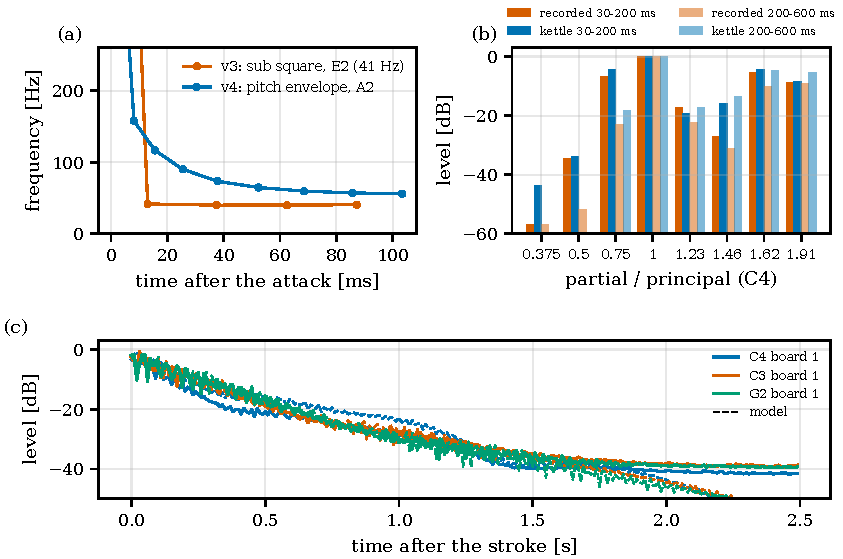
\includegraphics[width=\textwidth]{instr_drums.pdf}
\caption{Percussion (\file{tools/instrument\_figures.py}). (a) Kick pitch after the attack in the
behavioural model: version 3 (constant sub square) and version 4 (pitch envelope). (b) Kettle partials in two
time windows, relative to the principal: a recorded timpani (C4 stroke) and the kettle preset at C4 in the
model. (c) Kettle decay on board 1 (solid) and in the model (dashed) for C4, C3 and G2; below about
\SI{-40}{dB} the board's noise floor takes over (\file{docs/results/hw\_board1\_kettle.csv}).}\label{fig:drums}
\end{figure}

\subsection{Kettle: a modal timpani on the PWM DAC}\label{sec:kettle}
A drum's sound comes from the modes of its membrane: inharmonic partials, each with its own decay. The
analog voice has one periodic oscillator and one filter, so it cannot produce them. Modal synthesis can: a
bank of resonators, one per mode, excited by the strike. That needs an audio DAC, and the pulse output
can serve as one without any hardware change.

\paragraph{Pulse output as PWM DAC.} In DAC mode TIM2 counts up and down over 2 $\times$ 256 ticks, a
\SI{93.75}{kHz} carrier with 8-bit duty and pulses centred in the period. Centred pulses keep the signal from
also modulating the pulse position, which with simple up-counting PWM added a second harmonic of
\SI{0.6}{\percent} (S8). DMA1 channel~2 loads the channel-2 duty from a ring buffer on every timer update. In
this mode the update comes at both ends of the period, so each period's duty is stored twice, and the CPU
only fills the buffer. The DSP produces samples at \SI{15.625}{kHz} and interpolates linearly from one
sample to the next over the 6 carrier periods of a sample, which lowers the sampling images by about
\SI{23}{dB}. Each period's duty is quantised with first-order error feedback, which shapes the quantisation
noise towards the carrier, so the 8-bit DAC reaches about 10--11 bits in the audio band. The pulse pin feeds
the passive
mixer (\SI{470}{k\ohm} into \SI{10}{k\ohm}, then \SI{1}{\micro F}) and the ladder, which acts as the
reconstruction filter. The ladder's input pair sees only the two PWM levels, so its tanh characteristic does
not distort the duty-cycle code. S8 (Section~\ref{sec:s8}) checks the path in ngspice. Filter, resonance and
VCA keep working on the digital signal. The analog oscillator is parked in reset meanwhile, so a preset is
either analog or digital.

\paragraph{Modal synthesis.} Each stroke excites a bank of two-pole resonators, one per mode:
\[
  y[n] = 2r\cos\omega\; y[n-1] - r^2\, y[n-2] + b\, x[n],
\]
with $\omega$ from the mode's frequency, $r = e^{-1/(\tau f_s)}$ from its decay time $\tau$ and
$b = a\sin\omega$ for its level $a$. The excitation $x$ is a
raised-cosine mallet pulse of \SI{1}{ms} (a hard mallet; a shorter contact excites the upper modes more).
There are two banks, so two drums can ring at once. A stroke on a note that is still ringing adds to its bank,
as on a restruck drum; a new note takes a free or the oldest bank. The sum passes a cubic soft clipper
($1.5x - 0.5x^3$) before the encoder: rolls on a ringing drum add up, and the clipper rounds the rare peaks
instead of cutting them.

\paragraph{Fit to a recorded timpani.} The modes were fitted to a recorded F3--A3--C4 triad. In each stroke
the principal mode at the note carries the pitch. A mode at 0.75 times the note leads the first
\SI{30}{ms} and fades within about \SI{0.1}{s}, and a short thud lies at 0.375 times. Modes at 1.23, 1.46,
1.62 and 1.91 times colour the tone; the F and C strokes show the same ratios. The first fit read the strong
\SI{262}{Hz} partial of the C stroke as the octave of a C3 drum, which put every mode an octave too high.
The identical ratios in the F stroke resolved it.

The preset is deliberately harder and more metallic than the recording:
\begin{itemize}
  \item the \SI{1}{ms} mallet;
  \item the upper modes louder than in the recording, but still below the principal and decaying no
    slower, so the pitch stays on the note;
  \item four more high modes between 2.2 and 3.3 times the note;
  \item each strong mode doubled \SI{0.4}{\percent} higher, \SIrange{3}{8}{dB} weaker. A real membrane's
    modes are split into such pairs, and their beating gives the shimmer.
\end{itemize}
That makes 17 resonators. Figure~\ref{fig:drums}b compares the partials with the recording.

\paragraph{Firmware.} Signals are fixed point (Q24) with Q30 coefficients and use the CH32V006's hardware
multiplier; the coefficients are computed in floating point once per stroke. The main loop refills
128-sample halves of the ring, \SI{8.2}{ms} each. The CH32V003 and V002 have no multiplier or too little RAM
and keep the analog voice only. Four problems appeared on board 1:
\begin{itemize}
  \item \textbf{Stack overflow.} With the DSP state and the ring buffer, only 280 bytes of the 8\,KB RAM
    were left for the stack, which overwrote the patch and the CV values. The ring now shares the console's
    4\,KB capture buffer (captures are refused in DAC mode); 1.4\,KB remain.
  \item \textbf{Stalled control tick.} Selecting the kettle blocked interrupts for over \SI{1}{ms}. The
    SysTick handler schedules the next tick by adding to the compare value, which then lay in the past, so
    the next match came only after a counter wrap and the 1~kHz engine stopped. The handler now resynchronises
    when it falls behind, and the soft-float set-up no longer runs with interrupts blocked.
  \item \textbf{DSP too slow.} At first a refill took the whole half. The DSP rate was halved to
    \SI{15.625}{kHz} (the highest kettle mode is below \SI{1}{kHz}; the 4~kHz cutoff suppresses the sampling
    images). The excitation term is computed only during the mallet contact, and the refill loop runs from
    SRAM instead of flash. A refill now takes at most \SI{4.7}{ms} of the \SI{8.2}{ms} half.
  \item \textbf{Blocking console wait.} The console's \texttt{wait} command blocked the main loop and
    starved the DAC during test sequences; it now keeps the DAC fed.
\end{itemize}
The console command \texttt{dac} reports the DMA position, late refills and the longest refill.

\paragraph{Board 1 results.}
\begin{itemize}
  \item \textbf{DMA:} the transfer counter advances by 19 in \SI{100}{\micro s}, two updates per
    \SI{93.75}{kHz} period, so the TIM2 update request is served by DMA1 channel~2 as assumed, and the pitch
    is the same as with the first, edge-aligned version.
  \item \textbf{Centred pulses and interpolation:} against the first version (edge-aligned PWM, samples held)
    the share of 8 to \SI{20}{kHz} in a C3 stroke drops from $-38$ to \SI{-43.5}{dB}, and the noise in a
    decaying tail from 2.6 to \SI{2.2}{mV} rms.
  \item \textbf{Pitch:} C4, C3 and G2 strokes sound at 259.6, 129.9 and \SI{97.3}{Hz}: the note scaled by the
    board's \SI{-0.8}{\percent} clock, like every other pitch. In the recorded March part, 13 of 13 G2 strokes
    and 26 of 27 C3 strokes have their strongest partial on the note.
  \item \textbf{Decay:} within \SIrange{1}{4}{dB} of the model down to about \SI{-40}{dB}, where the board's
    noise floor takes over (Figure~\ref{fig:drums}c).
  \item \textbf{Timing:} no late refill in the test sequence, and the March take fits the common clock with
    \SI{3.3}{ms} rms, so the DSP kept up through the whole part.
  \item \textbf{Open:} a faint line at \SI{122}{Hz}, the buffer-half rate, \SI{61}{dB} below the take's peak.
    It is at the level of the board's noise floor and probably comes from the DSP's current bursts reaching
    the analog supply.
  \item \textbf{Carrier crosstalk:} the \SI{93.75}{kHz} carrier reaches the line out at about \SI{5.8}{mV}
    rms, far more than the filter path lets through (S8). Closing the VCA hardly changes it (\SI{4.9}{mV}), so
    it couples past the filter and the VCA, presumably from the PWM pin on the board. It is ultrasonic: in the
    audio band the line out stays at the board's noise floor (\SI{0.32}{mV} at 2 to \SI{8}{kHz}, measured at
    \SI{1}{MSa/s}). But a long scope take is sampled at only \SI{200}{kSa/s} (50\,Mpts for \SI{200}{s}),
    which folds the carrier's sidebands into the audio band; the board recordings therefore show about twice
    the true noise at 2 to \SI{8}{kHz}. A passive low-pass in front of the scope, or an audio interface,
    avoids that. A higher carrier would fold outside the audio band, but needs a faster DMA refill than the
    main loop allows.
  \item \textbf{Console traffic:} each console exchange blocks the main loop for about \SI{20}{ms}, longer
    than a buffer half; the recorder therefore no longer polls the console during a take.
\end{itemize}
The March recorded on board 1 uses the kettle (\file{docs/audio/pieces/march\_hw.mp3}). In the same folder,
\file{kettle\_model.mp3} plays the triad and the March pattern in the model.

% =====================================================================================================
\section{Verification and validation plan}\label{sec:vv}
Verification is organised in five levels (Table~\ref{tab:levels}). Levels L2 and L3 are designed to run
automatically. A host script drives the test firmware over the WCH-LinkE debug interface with
\file{minichlink}. It captures the audio loopback, computes spectra and compares them with limits derived
from the simulations. The results are stored as CSV next to the simulation data, so hardware and simulation
can be plotted together.

\begin{table}[h]
\centering\small
\caption{Verification levels.}\label{tab:levels}
\begin{tabularx}{\textwidth}{@{}l X X@{}}
\toprule
Level & Content & Method \\
\midrule
L0 & design verification & ngspice S1--S7 (done) \\
L1 & assembly and bring-up & DMM on the test points, current-limited supply \\
L2 & functional tests T1--T14 & test firmware + loopback ADC via \file{minichlink} (automated) \\
L3 & calibration & per-board constants stored in flash (automated) \\
L4 & validation & playing, listening, long-run stability (user) \\
\bottomrule
\end{tabularx}
\end{table}

\subsection{Bring-up}
Bring-up starts with the MCU not fitted, using a lab supply at \SI{9.0}{V} with a \SI{100}{mA} current limit
and the multimeter ground on one of the two scope-ground pins. The expected values in
Table~\ref{tab:bringup} are the DC operating point of the simulation netlist in exactly this state
(\file{sim/bringup/bringup\_op.py}, results in \file{docs/results/bringup\_expected.csv}). Without the MCU
its pins float:
\begin{itemize}
  \item \textbf{Linear CVs at zero}: the AMP, RES and VCA filter networks are pulled to \SI{0}{V} by their
    \SI{15}{k\ohm} last-stage resistor, so resonance is off and the VCA is shut.
  \item \textbf{Cutoff CV at VBIAS}: the cutoff network has no DC path of its own. XCUT\_IN floats up to
    VBIAS through the expo divider, both expo bases sit at VBIAS, and the ladder tail carries the expo
    reference current (about \SI{8}{\micro A}). Once the MCU drives the pin low, XCUT\_IN drops to about
    \SI{0.2}{V} and the tail current to nearly zero.
  \item \textbf{DCO held in reset}: the reset level shifter has no base drive, so the 2N7002 shorts the
    integrator capacitor and SAW sits at VREF.
  \item \textbf{Random shift-register state}: the 74HC595s power up with random outputs. Any number of the
    16 red LEDs (about \SI{0.68}{mA} each) may light, which moves the input current between the two values
    given for B3, and VTRIM can be anywhere between 0.4 and \SI{5}{V}.
\end{itemize}
The ladder bias taps are a divider from VP, so B7 is judged as the ratio to the measured VP. The other limits
leave room for resistor (\SI{1}{\percent}) and reference tolerances. A value outside its limit points to the
block on that test point's silkscreen frame.

\begin{table}[h]
\centering\small
\caption{Bring-up steps, MCU not fitted except B11--B12 (lab supply, current limit \SI{100}{mA}).
Expected values from the DC operating point of the netlist; board 1 measured at \SI{9}{V}, 2026-10-17, all
16 LEDs lit.}\label{tab:bringup}
\footnotesize\setlength{\tabcolsep}{4pt}
\begin{tabularx}{\textwidth}{@{}l >{\raggedright\arraybackslash}X l l l l@{}}
\toprule
\# & Step / test point & \SI{9}{V} in & \SI{12}{V} in & Limit (\SI{9}{V}) & Board 1 \\
\midrule
B1 & visual check; unpowered: no short VP, +5V to GND & -- & -- & -- & -- \\
B2 & reverse polarity, \SI{1}{s} & $I < \SI{1}{mA}$ & -- & pass & \SI{0}{mA} \\
B3 & input current & 14.8\,/\,\SI{25.7}{mA}\textsuperscript{a} & 15.9\,/\,\SI{26.8}{mA}\textsuperscript{a}
  & \SIrange{10}{35}{mA} & \SI{25}{mA}\textsuperscript{a} \\
B4 & VP & \SI{8.72}{V} & \SI{11.72}{V} & \SIrange{8.4}{8.9}{V} & \SI{8.57}{V} \\
B5 & +5V & \SI{5.00}{V} & \SI{5.00}{V} & \SIrange{4.8}{5.2}{V} & \SI{5.028}{V} \\
B6 & VREF & \SI{4.50}{V} & \SI{4.50}{V} & \SIrange{4.45}{4.55}{V} & \SI{4.53}{V} \\
B6a & VBIAS / V25 & 1.56 / \SI{2.50}{V} & 1.56 / \SI{2.50}{V} & $\pm$\SI{3}{\percent} & 1.57 / \SI{2.515}{V} \\
B7 & VB0 / VB2 / VB4 & 2.46 / 4.48 / \SI{6.50}{V} & 3.28 / 6.00 / \SI{8.72}{V} & & 2.39 / 4.32 / \SI{6.28}{V} \\
 & \quad as ratio to VP & 0.281 / 0.513 / 0.745 & & $\pm$\SI{3}{\percent} & 0.279 / 0.504 / 0.733 \\
B8 & TAIL & \SI{1.96}{V} & \SI{2.79}{V} & \SIrange{1.8}{2.1}{V} & \SI{1.88}{V} \\
B9 & LPF & \SI{4.50}{V} & \SI{4.50}{V} & \SIrange{4.3}{4.7}{V} & \SI{4.53}{V} \\
B10 & SAW / RESOUT / VCAOUT & \SI{4.50}{V} & \SI{4.50}{V} & \SIrange{4.3}{4.7}{V} & 4.52 / 4.52 / \SI{4.51}{V} \\
B10a & XAMP / XRES / XVCA & \SI{0}{V} & \SI{0}{V} & $<$ \SI{50}{mV} & 0 / 0 / \SI{0}{V} \\
B10b & XCUT\_IN & \SI{1.56}{V} & \SI{1.56}{V} & $\pm$\SI{3}{\percent} & \SI{1.57}{V} \\
B10c & VTRIM & 0.4 \ldots\ \SI{4.96}{V}\textsuperscript{b} & 0.4 \ldots\ \SI{4.96}{V}\textsuperscript{b} & -- & \SI{4.92}{V}\textsuperscript{b} \\
B11 & MCU fitted, \texttt{id} & -- & -- & answers & pass\textsuperscript{d} \\
B12 & current, MCU on & 20 \ldots\ \SI{31}{mA}\textsuperscript{c} & 21 \ldots\ \SI{32}{mA}\textsuperscript{c} & $<$ \SI{40}{mA} & \SI{25}{mA}\textsuperscript{e} \\
\bottomrule
\end{tabularx}\par\smallskip
\raggedright\textsuperscript{a} all LEDs off / all 16 LEDs on (random 74HC595 state at power-up); board 1: all on.\quad
\textsuperscript{b} random 74HC595 state; \SI{4.96}{V} = code 255.\quad \textsuperscript{c} MCU $\approx$ \SI{5}{mA}, 1 to 16 LEDs lit.\quad
\textsuperscript{d} CH32V006, firmware 0.1, reply \texttt{touchsynth 0.1 CH32V006}.\quad
\textsuperscript{e} firmware idle, all LEDs off; \SI{12}{V} not recorded.
\end{table}

\paragraph{Board 1 result (MCU not fitted).} B1--B10 pass. All three 74HC595s came up with every output high
(16 LEDs lit, VTRIM at code 255), which is a legitimate power-up state. Two observations:
\begin{itemize}
  \item \textbf{VP} is \SI{0.15}{V} below the simulation: the SS14 drops about \SI{0.43}{V} at \SI{25}{mA}
    instead of the model's \SI{0.28}{V} (or the supply leads drop part of it). The ratiometric parts of the
    design do not depend on it.
  \item \textbf{Ladder bias}: relative to VP, VB0 is \SI{0.9}{\percent} low and VB2 / VB4 are about
    \SI{1.7}{\percent} low. That is inside the limit but more than the resistor tolerance alone explains:
    roughly \SI{50}{\micro A} leaves the chain at the upper taps. TAIL follows VB0 minus one $V_\mathrm{BE}$
    and is consistent with it. To be watched in the VCF tests (T6--T8).
\end{itemize}
The first bring-up also corrected two simulation models: the 78L05 model drew only its quiescent current
from the input, and the TL072 macromodel drew about \SI{4}{mA} per amplifier instead of the datasheet
\SI{1.4}{mA}. Both are fixed in \file{sim/models/models.lib}. With them, the simulated input current with all
LEDs lit is \SI{25.7}{mA}, against \SI{25}{mA} measured. The first version of Table~\ref{tab:bringup} had also
driven the PWM nodes to \SI{0}{V}; that is the MCU-fitted state, not the floating one, and gave wrong
expectations for XCUT\_IN, TAIL and VBIAS.

\noindent After B11 the firmware drives the LEDs (octave display), sets the trim DAC to mid-scale (VTRIM
about \SI{2.7}{V}, loaded by the \SI{1}{M\ohm} injection resistor) and drives the cutoff PWM low (XCUT\_IN
about \SI{0.2}{V}). With \texttt{cv vca 0} and no note playing, B9--B10 should still hold.

\paragraph{Board 1 result (MCU fitted).} Board 1 carries a CH32V006. It was flashed with firmware 0.1 through a
WCH-LinkE and \file{minichlink} on a Linux host, which also carries the text console over SWIO
(\file{tools/synthtest.py}). B11 and B12 pass. The input current of \SI{25}{mA} with the firmware idle and all
LEDs off is about \SI{5}{mA} above the expected \SI{20}{mA}, which suggests that the MCU draws about
\SI{10}{mA} rather than the assumed \SI{5}{mA}; it is well inside the limit. Bring-up found one board defect
and several firmware faults, all fixed:
\begin{itemize}
  \item \textbf{PD4/PD5 solder bridge} (MCU pins 1 and 2, hand-soldered TSSOP). The loopback input read
    \SI{0}{V} instead of about \SI{2.7}{V}: \SI{4.5}{V} on the VCAOUT side of R109 and \SI{5}{mV} on the ADC
    side. Two console diagnostics located it: \texttt{adc <ch>} reads any ADC channel, and \texttt{latch
    <0|1>} holds the 74HC595 latch line (PD4) and reads port D back. With the latch line high, PD5 read
    4089 counts like PD4. After rework the loopback sits at 2209 counts (VCAOUT \SI{4.52}{V}).
  \item \textbf{Trim DAC MSB lost.} SRCLK of the LED/DAC shift-register chain is shared with mux select S1. A
    touch scan ended with it high, so the first rising edge was missing and the first bit shifted out, the DAC
    MSB, was lost. \texttt{hw\_leds\_dac} now pulls the clock low before the first bit (found in T1).
  \item \textbf{Loopback ADC on the V00x.} The ADC has to be re-armed before every conversion; without it the
    capture hung. The sample time was also shortened so that \SI{5}{\micro s} captures keep up, and the capture
    buffer holds 2048 samples on the V006.
  \item \textbf{Touch calibration.} The first noise estimate underflowed in unsigned arithmetic and gave some
    pads unreachable thresholds; it is now a signed deviation statistic over 64 scans. Pad~0 reads about
    550 counts low right after reset, which held key~C on; a \SI{300}{ms} warm-up scan precedes the
    calibration. During long recording sessions ghost touches still occurred, because the noise estimate
    came out as low as 48--96 counts on some boots. A threshold floor (\texttt{TOUCH\_MIN\_THR} = 200
    counts, against at least 486 counts for a real touch) and a two-scan debounce removed them.
  \item \textbf{Function-pad LEDs.} The LEDs next to SHIFT, $-$ and $+$ were never lit in normal playing:
    by design, the firmware used them only in edit mode or as the top of a value bar. The hardware was
    confirmed with \texttt{leds 0xe000}, after fixing the console's hex parser. The LEDs now light while
    their pad is touched.
\end{itemize}

\subsection{Functional tests}
\begin{longtable}{@{}l l p{6.2cm} p{3.9cm}@{}}
\caption{Functional tests (board 1: run from the PC with \file{tools/hwtest.py} over the console), limits
derived from the simulations.}\label{tab:tests}\\
\toprule ID & Block & Procedure & Pass limit (sim) \\ \midrule\endfirsthead
\toprule ID & Block & Procedure & Pass limit (sim) \\ \midrule\endhead
\bottomrule\endfoot
T1 & LEDs, 595 chain & walking one; trim DAC walk shifts VCAOUT DC monotonically & monotonic, $>$ \SI{20}{mV} span \\
T2 & touch & 256 readings per pad untouched; user touches each pad & $\sigma <$ 2\,LSB (V003) / 6\,LSB (V002); $\Delta > 10\sigma$ \\
T3 & touch scan & time a full 16-pad scan & $\geq$ \SI{200}{Hz} (sim 1.4\,kHz) \\
T4 & DCO pitch & loopback capture at C2, C4, C6 & $<$ 1\,cent \\
T5 & DCO amplitude & loopback amplitude C1--C8 & $\pm$\SI{5}{\percent} after calibration \\
T6 & VCF self-osc.\ threshold & ramp CV\sub{RES}, detect sustained oscillation & \SIrange{2.7}{3.5}{V} (sim 3.1\,V) \\
T7 & VCF tracking & self-oscillation frequency at CV\sub{CUT} = 1--4.5\,V & 2.05 $\pm$ 0.2\,oct/V \\
T8 & VCF low-pass & \SI{110}{Hz} saw, cutoff \SI{1}{kHz}, harmonic 10 vs.\ 1 & $\pm$\SI{3}{dB} of sim \\
T9 & VCA gain law & \SI{1}{kHz} saw, CV\sub{VCA} sweep & max.\ gain $\pm$\SI{2}{dB} of sim (+7.4\,dB) \\
T10 & VCA thump & CV\sub{VCA} steps without signal, before/after calibration & $<$ \SI{3}{mV} after (sim 0.6\,mV) \\
T11 & CV settling & VCA step seen at the loopback & 1\,\% in $<$ \SI{2.5}{ms} (sim 1.3\,ms) \\
T12 & hum and noise & VCA open, DCO off, spectrum & \SI{100}{Hz} $<$ sim + 6\,dB; broadband $< -60$\,dB \\
T14 & MIDI (if fitted) & note on/off, pitch bend, CC from a keyboard & all received \\
\end{longtable}

\subsection{Board 1 functional test results}\label{sec:board1}
The functional tests on board 1 (2026-10-17, \SI{9}{V} lab supply, room temperature) were run from the PC
with \file{tools/hwtest.py}. The script sends console commands (\texttt{cv}, \texttt{dco}, \texttt{trim},
\texttt{cap}, \texttt{capcv}) and evaluates the loopback captures; the on-chip \texttt{selftest} is not
implemented yet. The loopback ADC is 12-bit at PD5, which sees $0.6\times$ VCAOUT and is referenced to +5V
(\SI{5.028}{V}): one count is \SI{2.05}{mV} at VCAOUT. Captures have 2048 samples at
\SIrange{5}{100}{\micro s} per sample. All analog tests use the calibrated trim code 104. Evaluated data are in
\file{docs/results/hw\_board1\_*.csv}, the raw captures and console logs in \file{docs/results/hw\_board1/},
and Figures~\ref{fig:hw_dco}--\ref{fig:hw_hum} are generated by \file{tools/hw\_figures.py}.
Table~\ref{tab:board1} summarises the results. All executed tests pass, with two notes: the broadband noise
is marginal and the VCA has a slow tail when it opens. T3 and T14 were not run.

\begin{table}[ht]
\centering\small
\caption{Board 1 functional test results (2026-10-17). Levels in dB are relative to \SI{1.33}{V_{pp}}.}\label{tab:board1}
\footnotesize\setlength{\tabcolsep}{4pt}
\begin{tabularx}{\textwidth}{@{}l >{\raggedright\arraybackslash}X >{\raggedright\arraybackslash}p{2.9cm} >{\raggedright\arraybackslash}p{1.45cm}@{}}
\toprule
ID & Board 1 result & Limit (sim) & Verdict \\
\midrule
T1 & all 16 LEDs light; trim walk 0--255 moves the VCA-open level at VCAOUT monotonically over
  \SI{366}{mV} & monotonic, $>$ \SI{20}{mV} & pass \\
T2 & untouched $\sigma$ 20--28 counts (pads C--G) and 35--43 counts (G\#--$+$); touches 486--4233 counts,
  20--90\,$\sigma$; no ghost touch in a \SI{180}{s} log\textsuperscript{a} & $\Delta > 10\sigma$ & pass \\
T3 & not recorded & $\geq$ \SI{200}{Hz} & -- \\
T4 & $-0.28$ \ldots\ $+0.26$\,cent at 11 notes C2--C7, relative to the MCU clock\textsuperscript{b} & $<$ 1\,cent & pass \\
T5 & saw \SI{1.495}{V_{pp}} at VCAOUT, $-0.9$\,/\,$+1.2$\,\% over C2--C7, uncalibrated & $\pm$\SI{5}{\percent} & pass \\
T6 & onset between 3.05 and \SI{3.17}{V} (cutoff code 2211), oscillation at \SI{2.0}{kHz} & \SIrange{2.7}{3.5}{V} (3.1\,V) & pass \\
T7 & 2.01\,oct/V over CV\sub{CUT} = 0.49--\SI{4.02}{V} (\SI{89}{Hz} -- \SI{12.1}{kHz}), $\leq$ 45\,cent from a straight line
  & 2.05 $\pm$ 0.2\,oct/V & pass \\
T8 & harmonic 10 at \SI{-3.7}{dB} re harmonic 1; 4-pole fit $f_p$ = \SI{2077}{Hz} & $\pm$\SI{3}{dB} of
  sim\textsuperscript{c} & pass \\
T9 & gain law within $-0.23$ \ldots\ $+0.05$\,dB of S4 for CV\sub{VCA} = 0.25--\SI{5}{V}; off $\geq$ \SI{81}{dB}
  (measurement floor)\textsuperscript{d} & $\pm$\SI{2}{dB} & pass \\
T10 & thump at VCAOUT \SI{-33}{mV} at trim 128 (default), 0 $\pm$ \SI{2}{mV} at trim 104 & $<$ \SI{3}{mV} after cal.\ & pass \\
T11 & closing step: 1\,\% in \SI{1.17}{ms}; opening step: about 2\,\% left after \SI{1.5}{ms}, 1\,\% after
  \SI{12.8}{ms} & 1\,\% in $<$ \SI{2.5}{ms} (1.3\,ms) & pass\textsuperscript{e} \\
T12 & \SI{50}{Hz}: \SI{-82}{dB}, \SI{100}{Hz}: \SI{-79}{dB}; broadband (\SIrange{20}{5000}{Hz}) \SI{-54}{dB}
  with the VCA open, \SI{-55}{dB} closed & \SI{100}{Hz} $<$ \SI{-75}{dB}; broadband $< \SI{-60}{dB}$
  & hum pass, noise marginal \\
T14 & not tested & all received & -- \\
\bottomrule
\end{tabularx}\par\smallskip
\raggedright
\textsuperscript{a} A raw reading is the sum of 12 conversions, so the per-conversion $\sigma$ limit was not
evaluated; ghost touches seen later in long sessions led to the threshold floor (Section~\ref{sec:vv}, bring-up).\quad
\textsuperscript{b} DCO timer and capture share the HSI clock; the absolute pitch is \SI{14}{cent} flat (see text).\quad
\textsuperscript{c} an ideal 4-pole low-pass with the S3 cutoff for this code (\SI{1.0}{kHz} at \SI{-3}{dB}) gives
\SI{-3.5}{dB} at \SI{1.1}{kHz}.\quad
\textsuperscript{d} relative to full gain; the absolute maximum gain (S4: \SI{+7.4}{dB}) was not measured separately.\quad
\textsuperscript{e} for the CV network (closing step); the opening step has an additional slow component (see text).
\end{table}

\begin{figure}[ht]
\centering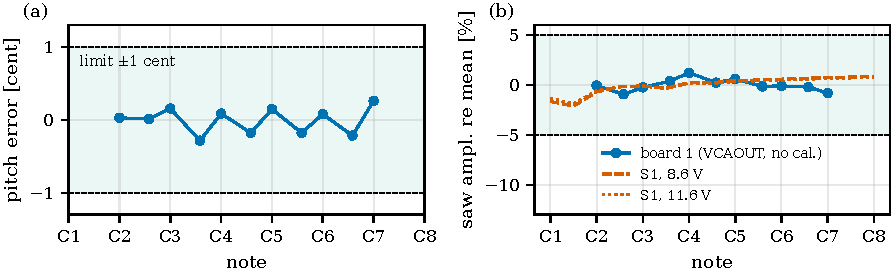
\includegraphics[width=\textwidth]{hw_board1_dco.pdf}
\caption{Board 1, T4/T5: (a) DCO pitch error from the loopback capture, relative to the MCU clock; (b) saw
amplitude at VCAOUT relative to its mean, without calibration, next to the S1 amplitude at both supply corners.}\label{fig:hw_dco}
\end{figure}

\begin{figure}[ht]
\centering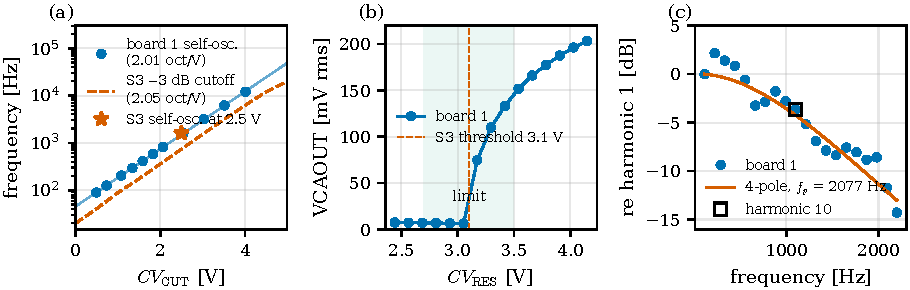
\includegraphics[width=\textwidth]{hw_board1_vcf.pdf}
\caption{Board 1, VCF: (a) T7, self-oscillation frequency versus CV\sub{CUT} with a straight-line fit, the S3
\SI{-3}{dB} cutoff and the S3 self-oscillation frequency at \SI{2.5}{V}; (b) T6, self-oscillation amplitude
versus CV\sub{RES} at the \SI{1}{kHz} cutoff code; (c) T8, response at the harmonics of a \SI{110}{Hz} saw
(filtered relative to the open filter) with a 4-pole fit.}\label{fig:hw_vcf}
\end{figure}

\begin{figure}[ht]
\centering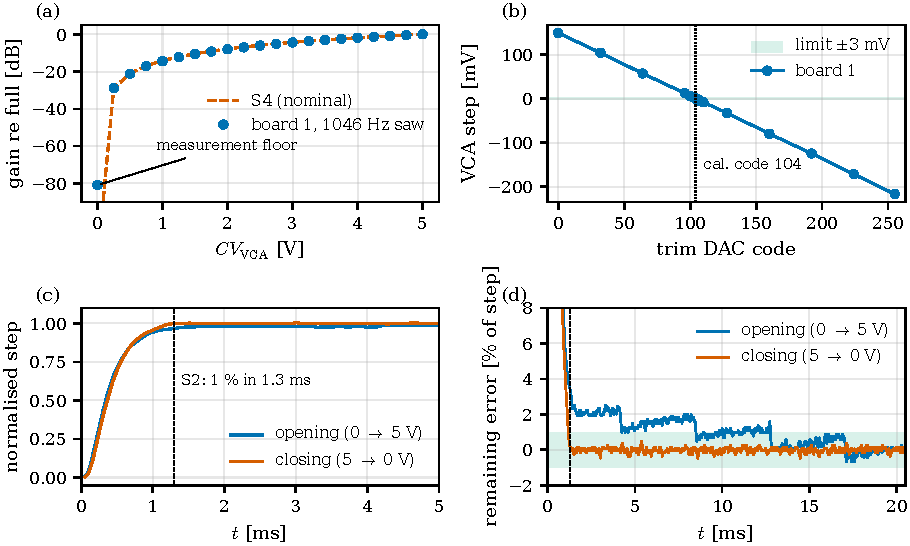
\includegraphics[width=\textwidth]{hw_board1_vca.pdf}
\caption{Board 1, VCA: (a) T9, gain law for a \SI{1046}{Hz} saw against S4; (b) T10, DC step at VCAOUT when
the VCA opens, versus trim code; (c) T11, CV\sub{VCA} step response at VCAOUT (trim 255 for a
\SI{220}{mV} DC step, 9-sample average), with the S2 settling time; (d) the same as remaining error.}\label{fig:hw_vca}
\end{figure}

\begin{figure}[ht]
\centering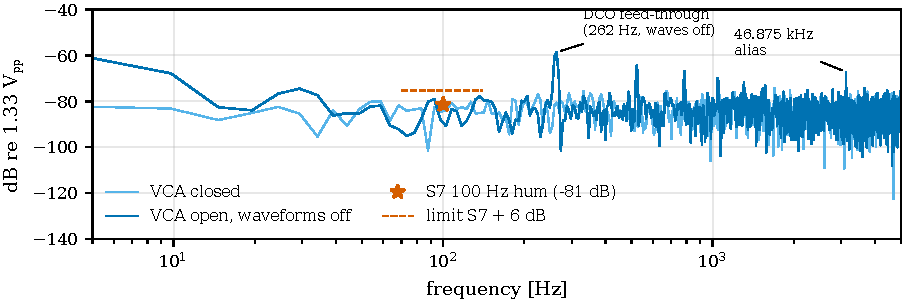
\includegraphics[width=\textwidth]{hw_board1_hum.pdf}
\caption{Board 1, T12: spectrum at VCAOUT (\SI{205}{ms} capture, \SI{10}{kS/s}, Hann window), VCA open and
closed, filter open, all waveforms off; the S7 hum value is for \SI{200}{mV_{pp}} input ripple.}\label{fig:hw_hum}
\end{figure}

\paragraph{Findings.}
\begin{itemize}
  \item \textbf{Oscillator and clock.} Pitch and saw amplitude are within limits without calibration
    (Figure~\ref{fig:hw_dco}); the amplitude spread ($-0.9$\,/\,$+1.2$\,\%) is similar to S1. Because the
    capture is timed by the same clock as the DCO, T4 checks the timer arithmetic but not the absolute pitch.
    From the scope recordings of the demo tunes (232 kick hits against the scope timebase), the HSI runs at
    \SI{47.62}{MHz}, \SI{-0.80}{\percent}. All pitches are therefore about \SI{14}{cent} flat and the tunes
    \SI{0.8}{\percent} slow until a clock trim is calibrated. Takes recorded up to an hour apart differed by up
    to \SI{0.1}{\percent}, the drift of the RC oscillator.
  \item \textbf{Filter.} Tracking, threshold and slope agree with S3 (Figure~\ref{fig:hw_vcf}). At
    CV\sub{CUT} = \SI{2.55}{V} the filter self-oscillates at \SI{1611}{Hz}; S3 gives \SI{1606}{Hz} at
    \SI{2.5}{V}, so board 1 is about 0.1\,octave lower at equal CV, which the cutoff calibration absorbs.
    The lowest sustained oscillation is \SI{89}{Hz} at \SI{0.49}{V}; at 0 and \SI{0.24}{V} only 5 and
    \SI{15}{mV_{rms}} remain. The harmonics scatter by about \SI{\pm2}{dB} around the 4-pole fit, and the
    fitted pole frequency (\SI{2077}{Hz}) agrees with the self-oscillation frequency at the same code (about
    \SI{2.0}{kHz}, T6). The low ladder bias seen in B7 has no visible effect.
  \item \textbf{VCA.} The gain law follows S4 within \SI{0.25}{dB} (Figure~\ref{fig:hw_vca}). The thump is
    linear in the trim code (\SI{-1.4}{mV} per code) and nulls at code 104, inside the expected 30--230. The
    firmware still boots with code 128, which leaves \SI{-33}{mV}, until the calibration store exists. The
    closing step settles to 1\,\% in \SI{1.17}{ms} (S2: \SI{1.3}{ms}). The opening step reaches about 2\,\%
    in \SI{1.5}{ms} and creeps in over another \SIrange{10}{15}{ms}. A linear RC network would settle alike in
    both directions, so the tail is most likely thermal: the VCA transistors warm up when their current jumps
    from zero. One ADC count is \SI{0.9}{\percent} of this step, so the tail is resolved only coarsely. At
    note-on it is a level creep of about 2\,\%.
  \item \textbf{Hum and noise.} The \SI{100}{Hz} hum (\SI{-79}{dB}) is at the noise floor with the lab
    supply; a test with mains adapters (V6) is still open. The broadband floor up to \SI{5}{kHz} is about
    \SI{-55}{dB} (total \SIrange{1.19}{1.29}{mV_{rms}} at VCAOUT with the discrete lines included, about
    \SI{-52}{dB}). It is nearly the same with the VCA closed, and the quantisation of the loopback alone
    (\SI{0.59}{mV_{rms}}) corresponds to \SI{-58}{dB}, so the loopback cannot verify the \SI{-60}{dB} goal.
    The scope recordings show a similar floor, about \SI{55}{dB} below the signal peaks in a \SI{24}{kHz}
    bandwidth. Two discrete lines appear in Figure~\ref{fig:hw_hum}: the running DCO's frequency and harmonics
    with all waveforms switched off and CV\sub{AMP} = 0 (feed-through with the VCA and filter open, up to
    \SI{-59}{dB}), and a line at \SI{3125}{Hz} in
    every capture, the \SI{46.875}{kHz} PWM and interrupt rate aliased by the \SI{10}{kS/s} capture.
\end{itemize}
Sound examples recorded from the line output with the oscilloscope (demo tunes, waveform switching and the
self-oscillating filter played as a scale) are in \file{docs/audio/hw\_board1/}.

\subsection{Calibration and validation}
\begin{itemize}
  \item \textbf{Calibration (L3)}: the calibration stores the DCO gain (expected 0.95--1.05), the cutoff
    scale and offset (from the self-oscillation frequency at two CV codes), the VCA trim code (expected
    30--230) and per-pad touch baselines and thresholds. The flash store is not implemented yet. Board 1
    values found manually: VCA trim code 104, HSI clock \SI{-0.80}{\percent} (pitch \SI{-14}{cent}); the DCO
    amplitude is within $-0.9$\,/\,$+1.2$\,\% without a gain constant. The touch baselines and thresholds are
    measured at every boot.
  \item \textbf{Validation (L4)}: covers reliable playing without ghost or double triggers, latency below
    \SI{10}{ms}, tuning stability, usability of the parameter UI, the sound compared with the
    behavioural-model examples, the demo tunes, hum with typical adapters, and MIDI.
\end{itemize}

\begin{table}[h]
\centering\small
\caption{Traceability from requirements to simulation and hardware tests.}\label{tab:trace}
\begin{tabular}{@{}l l l@{}}
\toprule
Requirement & Simulation & Hardware test \\
\midrule
DCO range and amplitude $\pm$\SI{5}{\percent} & S1 & T4, T5 \\
CV ripple and settling & S2 & T11 \\
VCF range, slope, resonance & S3 & T6, T7, T8 \\
VCA attenuation, thump & S4 & T9, T10 \\
Touch sensitivity and scan rate & S5 & T2, T3, V1, V2 \\
Complete voice & S6 & V5 \\
Power, hum & S7 & B2--B5, T12, V6 \\
\bottomrule
\end{tabular}
\end{table}

% =====================================================================================================
\section{Open points and risks}\label{sec:open}
\begin{itemize}
  \item \textbf{Accepted limitations.}
  \begin{itemize}
    \item Power-on pop at the line output (about \SI{3}{V}, \SI{0.3}{s}).
    \item Filter cutoff temperature drift of about $-13$\,cent/K. It could be compensated in firmware by
      re-tuning from the self-oscillation frequency, measured through the loopback.
  \end{itemize}
  \item \textbf{Not modelled in simulation.}
  \begin{itemize}
    \item The TL072 input common-mode limit. The design keeps all TL072 inputs at or above \SI{4}{V}.
    \item Noise. Board 1 measures about \SI{-55}{dB} broadband, at the limit of the loopback (T12).
    \item Transistor mismatch beyond the explicit cases.
    \item Thermal effects in the VCA pair: board 1 shows a slow 2\,\% tail when the VCA opens (T11).
    \item PCB parasitics, including key-to-key coupling of the touch pads and switching noise from the
      LEDs and shift registers. These are covered by T2 and T12.
  \end{itemize}
  \item \textbf{Open after board 1 bring-up} (Section~\ref{sec:board1}).
  \begin{itemize}
    \item \textbf{Calibration store (L3).} Not implemented. The firmware boots with trim code 128, which
      leaves a \SI{33}{mV} thump on board 1 (calibrated code 104). The pitch is \SI{14}{cent} flat from the
      \SI{-0.80}{\percent} HSI error, and the HSI drifts by up to \SI{0.1}{\percent}. The cutoff offset
      (about 0.1\,octave against S3) is not stored either.
    \item \textbf{Noise margin.} The broadband floor of about \SI{-55}{dB} misses the \SI{-60}{dB} goal, but
      the 12-bit loopback cannot resolve it (quantisation alone \SI{-58}{dB}). It should be measured at the
      line output with an audio interface.
    \item \textbf{VCA opening tail.} The level creeps by about 2\,\% over \SIrange{10}{15}{ms} after the
      fast part of the step, most likely thermally. Expected to be inaudible; confirm by listening (V5).
    \item \textbf{DCO feed-through.} With all waveforms off and the VCA open, the DCO frequency is still
      visible at up to \SI{-59}{dB}.
    \item \textbf{Not yet tested.} B12 at \SI{12}{V}, T3 (scan rate), T14 (MIDI), the on-chip
      \texttt{selftest}, hum with mains adapters (V6) and the L4 validation in general.
    \item \textbf{DAC mode} (Section~\ref{sec:kettle}). A faint \SI{122}{Hz} line (the buffer-half rate,
      \SI{-61}{dB} re peak), probably the DSP's current bursts on the supply; smaller buffer halves would move
      it up and spread the load. The kettle uses up to about half of the CPU and leaves 1.4\,KB of stack, so
      more digital voices need care. A firmware routine that blocks the main loop for more than a buffer half
      (\SI{8.2}{ms}) would starve the DAC; a console exchange does (about \SI{20}{ms}).
    \item \textbf{For a board revision: PWM carrier crosstalk.} In DAC mode about \SI{5.8}{mV} of the
      \SI{93.75}{kHz} carrier reaches the line out past the filter and the VCA (Section~\ref{sec:kettle}).
      Inaudible, but it folds into the audio band of sampled recordings and can upset amplifiers or
      converters downstream. Slow the PULSE edges at the pin (series resistor and a small capacitor to ground,
      corner well above the carrier), and review the routing and ground return of the PULSE trace and its
      neighbours to the output stage. The firmware keeps the \SI{93.75}{kHz} carrier for now; a higher carrier
      (\SI{375}{kHz}, 6-bit, still centred, interpolated and noise-shaped) would fold outside the audio band,
      but needs the DMA refill moved into an interrupt.
  \end{itemize}
  \item \textbf{Touch sensitivity on the 4-layer board} (resolved on board 1). Real touches give 486 to 4233
    counts against an untouched $\sigma$ of 20--43 counts. The thresholds need a floor of 200 counts and a
    two-scan debounce, because the boot-time noise estimate is sometimes too low (Section~\ref{sec:vv}).
  \item \textbf{CH32V006 pinout} (resolved). The V006 datasheet (V2.0, table 2-1-1, V006F8P7) gives the same
    TSSOP-20 pin numbers and the same \texttt{\_2} remap functions as the CH32V002. The reset pin is PD7; PA4 is
    bonded to PD7 inside the package and is never used. Board 1 carries a CH32V006.
  \item \textbf{Assembly.} Check the orientation of the SOT-23/SOT-363 transistors, the diode and the LEDs
    at the first inspection. Hand-solder the TSSOP-20 MCU and check pins 1--2 (PD4/PD5) for a bridge: board 1
    had one, which held the loopback input low.
  \item \textbf{Documentation.} The specification (\file{docs/spec.md}) and the verification plan still
    describe some pre-layout details (two layers, test pads on the bottom side). This report reflects the
    design as ordered.
\end{itemize}

% =====================================================================================================
\appendix
\section{Schematic}\label{app:sch}
The following pages reproduce the KiCad schematic (\file{docs/touchsynth\_schematic.pdf}) scaled to A4. The
PDF is vector graphics and can be zoomed.

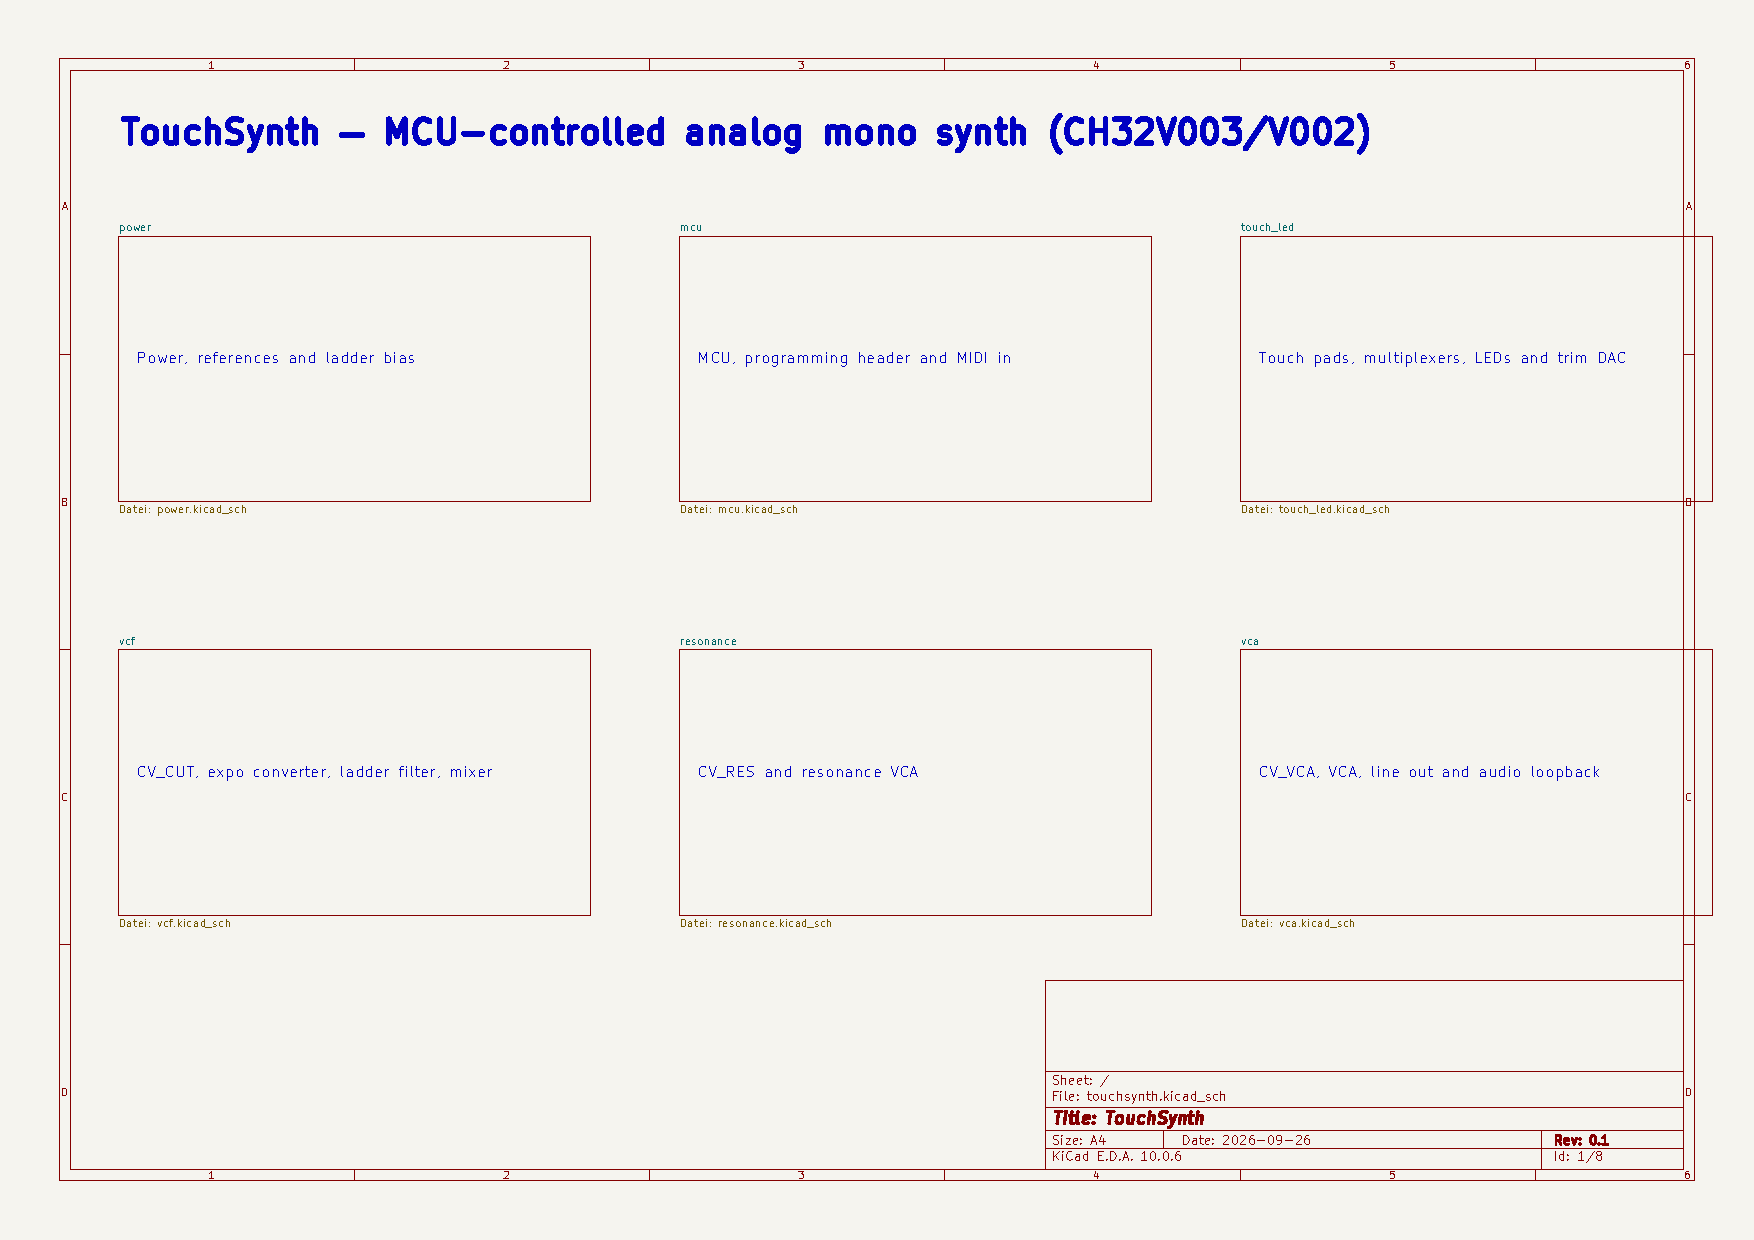
\includepdf[pages=-,landscape,fitpaper=false,scale=0.95,pagecommand={\thispagestyle{fancy}}]{../touchsynth_schematic.pdf}

\section{Reproducing the design}
\begin{footnotesize}
\begin{verbatim}
cd sim/s1_dco && python s1_dco.py      # likewise s2_cv ... s8_dac (order: S1, S3, S4, S6)
cd sim/behav && python validate.py && python examples.py
cd hw && python gen_sch2.py && python check_netlist.py && python check_sim.py
cd hw && <KiCad python> gen_pcb.py --route  # placement, routing, fill, stitching
cd hw && python fab.py                      # gerbers, BOM, CPL
cd docs/report && python gen_tables.py && latexmk -pdf touchsynth_report.tex
cd firmware/touchsynth && python gen_tables.py && make TARGET_MCU=CH32V006 && make flash
# bench (lab setup in tools/lab.conf, from tools/lab.conf.example):
cd tools && python hwtest.py dco      # also vcf, vca, settle, hum, lpf
cd tools && python hw_figures.py && python instrument_figures.py <timpani recording>
./record_parts.sh 200 march_timp:15   # on the lab PC: one part per take
cd tools && python mix_parts.py hw <takes> march && python suite.py hw <takes>
\end{verbatim}
\end{footnotesize}

\end{document}
